
\documentclass[10pt]{article} % For LaTeX2e
\usepackage{tmlr}
% If accepted, instead use the following line for the camera-ready submission:
%\usepackage[accepted]{tmlr}
% To de-anonymize and remove mentions to TMLR (for example for posting to preprint servers), instead use the following:
%\usepackage[preprint]{tmlr}

% Optional math commands from https://github.com/goodfeli/dlbook_notation.
%%%%% NEW MATH DEFINITIONS %%%%%

\usepackage{amsmath,amsfonts,bm}

% Mark sections of captions for referring to divisions of figures
\newcommand{\figleft}{{\em (Left)}}
\newcommand{\figcenter}{{\em (Center)}}
\newcommand{\figright}{{\em (Right)}}
\newcommand{\figtop}{{\em (Top)}}
\newcommand{\figbottom}{{\em (Bottom)}}
\newcommand{\captiona}{{\em (a)}}
\newcommand{\captionb}{{\em (b)}}
\newcommand{\captionc}{{\em (c)}}
\newcommand{\captiond}{{\em (d)}}

% Highlight a newly defined term
\newcommand{\newterm}[1]{{\bf #1}}


% Figure reference, lower-case.
\def\figref#1{figure~\ref{#1}}
% Figure reference, capital. For start of sentence
\def\Figref#1{Figure~\ref{#1}}
\def\twofigref#1#2{figures \ref{#1} and \ref{#2}}
\def\quadfigref#1#2#3#4{figures \ref{#1}, \ref{#2}, \ref{#3} and \ref{#4}}
% Section reference, lower-case.
\def\secref#1{section~\ref{#1}}
% Section reference, capital.
\def\Secref#1{Section~\ref{#1}}
% Reference to two sections.
\def\twosecrefs#1#2{sections \ref{#1} and \ref{#2}}
% Reference to three sections.
\def\secrefs#1#2#3{sections \ref{#1}, \ref{#2} and \ref{#3}}
% Reference to an equation, lower-case.
\def\eqref#1{equation~\ref{#1}}
% Reference to an equation, upper case
\def\Eqref#1{Equation~\ref{#1}}
% A raw reference to an equation---avoid using if possible
\def\plaineqref#1{\ref{#1}}
% Reference to a chapter, lower-case.
\def\chapref#1{chapter~\ref{#1}}
% Reference to an equation, upper case.
\def\Chapref#1{Chapter~\ref{#1}}
% Reference to a range of chapters
\def\rangechapref#1#2{chapters\ref{#1}--\ref{#2}}
% Reference to an algorithm, lower-case.
\def\algref#1{algorithm~\ref{#1}}
% Reference to an algorithm, upper case.
\def\Algref#1{Algorithm~\ref{#1}}
\def\twoalgref#1#2{algorithms \ref{#1} and \ref{#2}}
\def\Twoalgref#1#2{Algorithms \ref{#1} and \ref{#2}}
% Reference to a part, lower case
\def\partref#1{part~\ref{#1}}
% Reference to a part, upper case
\def\Partref#1{Part~\ref{#1}}
\def\twopartref#1#2{parts \ref{#1} and \ref{#2}}

\def\ceil#1{\lceil #1 \rceil}
\def\floor#1{\lfloor #1 \rfloor}
\def\1{\bm{1}}
\newcommand{\train}{\mathcal{D}}
\newcommand{\valid}{\mathcal{D_{\mathrm{valid}}}}
\newcommand{\test}{\mathcal{D_{\mathrm{test}}}}

\def\eps{{\epsilon}}


% Random variables
\def\reta{{\textnormal{$\eta$}}}
\def\ra{{\textnormal{a}}}
\def\rb{{\textnormal{b}}}
\def\rc{{\textnormal{c}}}
\def\rd{{\textnormal{d}}}
\def\re{{\textnormal{e}}}
\def\rf{{\textnormal{f}}}
\def\rg{{\textnormal{g}}}
\def\rh{{\textnormal{h}}}
\def\ri{{\textnormal{i}}}
\def\rj{{\textnormal{j}}}
\def\rk{{\textnormal{k}}}
\def\rl{{\textnormal{l}}}
% rm is already a command, just don't name any random variables m
\def\rn{{\textnormal{n}}}
\def\ro{{\textnormal{o}}}
\def\rp{{\textnormal{p}}}
\def\rq{{\textnormal{q}}}
\def\rr{{\textnormal{r}}}
\def\rs{{\textnormal{s}}}
\def\rt{{\textnormal{t}}}
\def\ru{{\textnormal{u}}}
\def\rv{{\textnormal{v}}}
\def\rw{{\textnormal{w}}}
\def\rx{{\textnormal{x}}}
\def\ry{{\textnormal{y}}}
\def\rz{{\textnormal{z}}}

% Random vectors
\def\rvepsilon{{\mathbf{\epsilon}}}
\def\rvtheta{{\mathbf{\theta}}}
\def\rva{{\mathbf{a}}}
\def\rvb{{\mathbf{b}}}
\def\rvc{{\mathbf{c}}}
\def\rvd{{\mathbf{d}}}
\def\rve{{\mathbf{e}}}
\def\rvf{{\mathbf{f}}}
\def\rvg{{\mathbf{g}}}
\def\rvh{{\mathbf{h}}}
\def\rvu{{\mathbf{i}}}
\def\rvj{{\mathbf{j}}}
\def\rvk{{\mathbf{k}}}
\def\rvl{{\mathbf{l}}}
\def\rvm{{\mathbf{m}}}
\def\rvn{{\mathbf{n}}}
\def\rvo{{\mathbf{o}}}
\def\rvp{{\mathbf{p}}}
\def\rvq{{\mathbf{q}}}
\def\rvr{{\mathbf{r}}}
\def\rvs{{\mathbf{s}}}
\def\rvt{{\mathbf{t}}}
\def\rvu{{\mathbf{u}}}
\def\rvv{{\mathbf{v}}}
\def\rvw{{\mathbf{w}}}
\def\rvx{{\mathbf{x}}}
\def\rvy{{\mathbf{y}}}
\def\rvz{{\mathbf{z}}}

% Elements of random vectors
\def\erva{{\textnormal{a}}}
\def\ervb{{\textnormal{b}}}
\def\ervc{{\textnormal{c}}}
\def\ervd{{\textnormal{d}}}
\def\erve{{\textnormal{e}}}
\def\ervf{{\textnormal{f}}}
\def\ervg{{\textnormal{g}}}
\def\ervh{{\textnormal{h}}}
\def\ervi{{\textnormal{i}}}
\def\ervj{{\textnormal{j}}}
\def\ervk{{\textnormal{k}}}
\def\ervl{{\textnormal{l}}}
\def\ervm{{\textnormal{m}}}
\def\ervn{{\textnormal{n}}}
\def\ervo{{\textnormal{o}}}
\def\ervp{{\textnormal{p}}}
\def\ervq{{\textnormal{q}}}
\def\ervr{{\textnormal{r}}}
\def\ervs{{\textnormal{s}}}
\def\ervt{{\textnormal{t}}}
\def\ervu{{\textnormal{u}}}
\def\ervv{{\textnormal{v}}}
\def\ervw{{\textnormal{w}}}
\def\ervx{{\textnormal{x}}}
\def\ervy{{\textnormal{y}}}
\def\ervz{{\textnormal{z}}}

% Random matrices
\def\rmA{{\mathbf{A}}}
\def\rmB{{\mathbf{B}}}
\def\rmC{{\mathbf{C}}}
\def\rmD{{\mathbf{D}}}
\def\rmE{{\mathbf{E}}}
\def\rmF{{\mathbf{F}}}
\def\rmG{{\mathbf{G}}}
\def\rmH{{\mathbf{H}}}
\def\rmI{{\mathbf{I}}}
\def\rmJ{{\mathbf{J}}}
\def\rmK{{\mathbf{K}}}
\def\rmL{{\mathbf{L}}}
\def\rmM{{\mathbf{M}}}
\def\rmN{{\mathbf{N}}}
\def\rmO{{\mathbf{O}}}
\def\rmP{{\mathbf{P}}}
\def\rmQ{{\mathbf{Q}}}
\def\rmR{{\mathbf{R}}}
\def\rmS{{\mathbf{S}}}
\def\rmT{{\mathbf{T}}}
\def\rmU{{\mathbf{U}}}
\def\rmV{{\mathbf{V}}}
\def\rmW{{\mathbf{W}}}
\def\rmX{{\mathbf{X}}}
\def\rmY{{\mathbf{Y}}}
\def\rmZ{{\mathbf{Z}}}

% Elements of random matrices
\def\ermA{{\textnormal{A}}}
\def\ermB{{\textnormal{B}}}
\def\ermC{{\textnormal{C}}}
\def\ermD{{\textnormal{D}}}
\def\ermE{{\textnormal{E}}}
\def\ermF{{\textnormal{F}}}
\def\ermG{{\textnormal{G}}}
\def\ermH{{\textnormal{H}}}
\def\ermI{{\textnormal{I}}}
\def\ermJ{{\textnormal{J}}}
\def\ermK{{\textnormal{K}}}
\def\ermL{{\textnormal{L}}}
\def\ermM{{\textnormal{M}}}
\def\ermN{{\textnormal{N}}}
\def\ermO{{\textnormal{O}}}
\def\ermP{{\textnormal{P}}}
\def\ermQ{{\textnormal{Q}}}
\def\ermR{{\textnormal{R}}}
\def\ermS{{\textnormal{S}}}
\def\ermT{{\textnormal{T}}}
\def\ermU{{\textnormal{U}}}
\def\ermV{{\textnormal{V}}}
\def\ermW{{\textnormal{W}}}
\def\ermX{{\textnormal{X}}}
\def\ermY{{\textnormal{Y}}}
\def\ermZ{{\textnormal{Z}}}

% Vectors
\def\vzero{{\bm{0}}}
\def\vone{{\bm{1}}}
\def\vmu{{\bm{\mu}}}
\def\vtheta{{\bm{\theta}}}
\def\va{{\bm{a}}}
\def\vb{{\bm{b}}}
\def\vc{{\bm{c}}}
\def\vd{{\bm{d}}}
\def\ve{{\bm{e}}}
\def\vf{{\bm{f}}}
\def\vg{{\bm{g}}}
\def\vh{{\bm{h}}}
\def\vi{{\bm{i}}}
\def\vj{{\bm{j}}}
\def\vk{{\bm{k}}}
\def\vl{{\bm{l}}}
\def\vm{{\bm{m}}}
\def\vn{{\bm{n}}}
\def\vo{{\bm{o}}}
\def\vp{{\bm{p}}}
\def\vq{{\bm{q}}}
\def\vr{{\bm{r}}}
\def\vs{{\bm{s}}}
\def\vt{{\bm{t}}}
\def\vu{{\bm{u}}}
\def\vv{{\bm{v}}}
\def\vw{{\bm{w}}}
\def\vx{{\bm{x}}}
\def\vy{{\bm{y}}}
\def\vz{{\bm{z}}}

% Elements of vectors
\def\evalpha{{\alpha}}
\def\evbeta{{\beta}}
\def\evepsilon{{\epsilon}}
\def\evlambda{{\lambda}}
\def\evomega{{\omega}}
\def\evmu{{\mu}}
\def\evpsi{{\psi}}
\def\evsigma{{\sigma}}
\def\evtheta{{\theta}}
\def\eva{{a}}
\def\evb{{b}}
\def\evc{{c}}
\def\evd{{d}}
\def\eve{{e}}
\def\evf{{f}}
\def\evg{{g}}
\def\evh{{h}}
\def\evi{{i}}
\def\evj{{j}}
\def\evk{{k}}
\def\evl{{l}}
\def\evm{{m}}
\def\evn{{n}}
\def\evo{{o}}
\def\evp{{p}}
\def\evq{{q}}
\def\evr{{r}}
\def\evs{{s}}
\def\evt{{t}}
\def\evu{{u}}
\def\evv{{v}}
\def\evw{{w}}
\def\evx{{x}}
\def\evy{{y}}
\def\evz{{z}}

% Matrix
\def\mA{{\bm{A}}}
\def\mB{{\bm{B}}}
\def\mC{{\bm{C}}}
\def\mD{{\bm{D}}}
\def\mE{{\bm{E}}}
\def\mF{{\bm{F}}}
\def\mG{{\bm{G}}}
\def\mH{{\bm{H}}}
\def\mI{{\bm{I}}}
\def\mJ{{\bm{J}}}
\def\mK{{\bm{K}}}
\def\mL{{\bm{L}}}
\def\mM{{\bm{M}}}
\def\mN{{\bm{N}}}
\def\mO{{\bm{O}}}
\def\mP{{\bm{P}}}
\def\mQ{{\bm{Q}}}
\def\mR{{\bm{R}}}
\def\mS{{\bm{S}}}
\def\mT{{\bm{T}}}
\def\mU{{\bm{U}}}
\def\mV{{\bm{V}}}
\def\mW{{\bm{W}}}
\def\mX{{\bm{X}}}
\def\mY{{\bm{Y}}}
\def\mZ{{\bm{Z}}}
\def\mBeta{{\bm{\beta}}}
\def\mPhi{{\bm{\Phi}}}
\def\mLambda{{\bm{\Lambda}}}
\def\mSigma{{\bm{\Sigma}}}

% Tensor
\DeclareMathAlphabet{\mathsfit}{\encodingdefault}{\sfdefault}{m}{sl}
\SetMathAlphabet{\mathsfit}{bold}{\encodingdefault}{\sfdefault}{bx}{n}
\newcommand{\tens}[1]{\bm{\mathsfit{#1}}}
\def\tA{{\tens{A}}}
\def\tB{{\tens{B}}}
\def\tC{{\tens{C}}}
\def\tD{{\tens{D}}}
\def\tE{{\tens{E}}}
\def\tF{{\tens{F}}}
\def\tG{{\tens{G}}}
\def\tH{{\tens{H}}}
\def\tI{{\tens{I}}}
\def\tJ{{\tens{J}}}
\def\tK{{\tens{K}}}
\def\tL{{\tens{L}}}
\def\tM{{\tens{M}}}
\def\tN{{\tens{N}}}
\def\tO{{\tens{O}}}
\def\tP{{\tens{P}}}
\def\tQ{{\tens{Q}}}
\def\tR{{\tens{R}}}
\def\tS{{\tens{S}}}
\def\tT{{\tens{T}}}
\def\tU{{\tens{U}}}
\def\tV{{\tens{V}}}
\def\tW{{\tens{W}}}
\def\tX{{\tens{X}}}
\def\tY{{\tens{Y}}}
\def\tZ{{\tens{Z}}}


% Graph
\def\gA{{\mathcal{A}}}
\def\gB{{\mathcal{B}}}
\def\gC{{\mathcal{C}}}
\def\gD{{\mathcal{D}}}
\def\gE{{\mathcal{E}}}
\def\gF{{\mathcal{F}}}
\def\gG{{\mathcal{G}}}
\def\gH{{\mathcal{H}}}
\def\gI{{\mathcal{I}}}
\def\gJ{{\mathcal{J}}}
\def\gK{{\mathcal{K}}}
\def\gL{{\mathcal{L}}}
\def\gM{{\mathcal{M}}}
\def\gN{{\mathcal{N}}}
\def\gO{{\mathcal{O}}}
\def\gP{{\mathcal{P}}}
\def\gQ{{\mathcal{Q}}}
\def\gR{{\mathcal{R}}}
\def\gS{{\mathcal{S}}}
\def\gT{{\mathcal{T}}}
\def\gU{{\mathcal{U}}}
\def\gV{{\mathcal{V}}}
\def\gW{{\mathcal{W}}}
\def\gX{{\mathcal{X}}}
\def\gY{{\mathcal{Y}}}
\def\gZ{{\mathcal{Z}}}

% Sets
\def\sA{{\mathbb{A}}}
\def\sB{{\mathbb{B}}}
\def\sC{{\mathbb{C}}}
\def\sD{{\mathbb{D}}}
% Don't use a set called E, because this would be the same as our symbol
% for expectation.
\def\sF{{\mathbb{F}}}
\def\sG{{\mathbb{G}}}
\def\sH{{\mathbb{H}}}
\def\sI{{\mathbb{I}}}
\def\sJ{{\mathbb{J}}}
\def\sK{{\mathbb{K}}}
\def\sL{{\mathbb{L}}}
\def\sM{{\mathbb{M}}}
\def\sN{{\mathbb{N}}}
\def\sO{{\mathbb{O}}}
\def\sP{{\mathbb{P}}}
\def\sQ{{\mathbb{Q}}}
\def\sR{{\mathbb{R}}}
\def\sS{{\mathbb{S}}}
\def\sT{{\mathbb{T}}}
\def\sU{{\mathbb{U}}}
\def\sV{{\mathbb{V}}}
\def\sW{{\mathbb{W}}}
\def\sX{{\mathbb{X}}}
\def\sY{{\mathbb{Y}}}
\def\sZ{{\mathbb{Z}}}

% Entries of a matrix
\def\emLambda{{\Lambda}}
\def\emA{{A}}
\def\emB{{B}}
\def\emC{{C}}
\def\emD{{D}}
\def\emE{{E}}
\def\emF{{F}}
\def\emG{{G}}
\def\emH{{H}}
\def\emI{{I}}
\def\emJ{{J}}
\def\emK{{K}}
\def\emL{{L}}
\def\emM{{M}}
\def\emN{{N}}
\def\emO{{O}}
\def\emP{{P}}
\def\emQ{{Q}}
\def\emR{{R}}
\def\emS{{S}}
\def\emT{{T}}
\def\emU{{U}}
\def\emV{{V}}
\def\emW{{W}}
\def\emX{{X}}
\def\emY{{Y}}
\def\emZ{{Z}}
\def\emSigma{{\Sigma}}

% entries of a tensor
% Same font as tensor, without \bm wrapper
\newcommand{\etens}[1]{\mathsfit{#1}}
\def\etLambda{{\etens{\Lambda}}}
\def\etA{{\etens{A}}}
\def\etB{{\etens{B}}}
\def\etC{{\etens{C}}}
\def\etD{{\etens{D}}}
\def\etE{{\etens{E}}}
\def\etF{{\etens{F}}}
\def\etG{{\etens{G}}}
\def\etH{{\etens{H}}}
\def\etI{{\etens{I}}}
\def\etJ{{\etens{J}}}
\def\etK{{\etens{K}}}
\def\etL{{\etens{L}}}
\def\etM{{\etens{M}}}
\def\etN{{\etens{N}}}
\def\etO{{\etens{O}}}
\def\etP{{\etens{P}}}
\def\etQ{{\etens{Q}}}
\def\etR{{\etens{R}}}
\def\etS{{\etens{S}}}
\def\etT{{\etens{T}}}
\def\etU{{\etens{U}}}
\def\etV{{\etens{V}}}
\def\etW{{\etens{W}}}
\def\etX{{\etens{X}}}
\def\etY{{\etens{Y}}}
\def\etZ{{\etens{Z}}}

% The true underlying data generating distribution
\newcommand{\pdata}{p_{\rm{data}}}
% The empirical distribution defined by the training set
\newcommand{\ptrain}{\hat{p}_{\rm{data}}}
\newcommand{\Ptrain}{\hat{P}_{\rm{data}}}
% The model distribution
\newcommand{\pmodel}{p_{\rm{model}}}
\newcommand{\Pmodel}{P_{\rm{model}}}
\newcommand{\ptildemodel}{\tilde{p}_{\rm{model}}}
% Stochastic autoencoder distributions
\newcommand{\pencode}{p_{\rm{encoder}}}
\newcommand{\pdecode}{p_{\rm{decoder}}}
\newcommand{\precons}{p_{\rm{reconstruct}}}

\newcommand{\laplace}{\mathrm{Laplace}} % Laplace distribution

\newcommand{\E}{\mathbb{E}}
\newcommand{\Ls}{\mathcal{L}}
\newcommand{\R}{\mathbb{R}}
\newcommand{\emp}{\tilde{p}}
\newcommand{\lr}{\alpha}
\newcommand{\reg}{\lambda}
\newcommand{\rect}{\mathrm{rectifier}}
\newcommand{\softmax}{\mathrm{softmax}}
\newcommand{\sigmoid}{\sigma}
\newcommand{\softplus}{\zeta}
\newcommand{\KL}{D_{\mathrm{KL}}}
\newcommand{\Var}{\mathrm{Var}}
\newcommand{\standarderror}{\mathrm{SE}}
\newcommand{\Cov}{\mathrm{Cov}}
% Wolfram Mathworld says $L^2$ is for function spaces and $\ell^2$ is for vectors
% But then they seem to use $L^2$ for vectors throughout the site, and so does
% wikipedia.
\newcommand{\normlzero}{L^0}
\newcommand{\normlone}{L^1}
\newcommand{\normltwo}{L^2}
\newcommand{\normlp}{L^p}
\newcommand{\normmax}{L^\infty}

\newcommand{\parents}{Pa} % See usage in notation.tex. Chosen to match Daphne's book.

\DeclareMathOperator*{\argmax}{arg\,max}
\DeclareMathOperator*{\argmin}{arg\,min}

\DeclareMathOperator{\sign}{sign}
\DeclareMathOperator{\Tr}{Tr}
\let\ab\allowbreak


\usepackage{hyperref}
\usepackage{url}
\usepackage[ruled,vlined]{algorithm2e}
\usepackage{multirow}
\usepackage{subcaption}
\usepackage{graphicx}
\usepackage{enumitem}
\usepackage{placeins}  % preamble
\usepackage[font=small,skip=4pt]{caption}
\usepackage{float}   % for [H]
\usepackage{placeins}


% \usepackage[pagenumbers]{cvpr} % To force page numbers, e.g. for an arXiv version
\usepackage{booktabs}
\usepackage{xcolor}

\title{HyperDG: Does Per-Domain Hyperbolic Curvature Help Domain Generalization? \\ A Controlled Test on a Pretrained Backbone}

% Authors must not appear in the submitted version. They should be hidden
% as long as the tmlr package is used without the [accepted] or [preprint] options.
% Non-anonymous submissions will be rejected without review.

\author{\name Kyunghyun Cho \email kyunghyun.cho@nyu.edu \\
      \addr Department of Computer Science\\
      University of New York
      \AND
      \name Raia Hadsell \email raia@google.com \\
      \addr DeepMind
      \AND
      \name Hugo Larochelle \email hugolarochelle@google.com\\
      \addr Mila, Universit\'e de Montr\'eal \\
      Google Research\\
      CIFAR Fellow}

% The \author macro works with any number of authors. Use \AND 
% to separate the names and addresses of multiple authors.

\newcommand{\fix}{\marginpar{FIX}}
\newcommand{\new}{\marginpar{NEW}}

\def\month{MM}  % Insert correct month for camera-ready version
\def\year{YYYY} % Insert correct year for camera-ready version
\def\openreview{\url{https://openreview.net/forum?id=XXXX}} % Insert correct link to OpenReview for camera-ready version


\begin{document}


\maketitle

\begin{abstract}
A growing line of work motivates non-Euclidean representation spaces for domain
generalization (DG), with the intuition that real data manifolds are inherently
curved and that per-domain geometric structure must be respected to obtain
transferable features. We test this intuition rigorously by building
\textbf{HyperDG}, a multi-source DG framework that models each domain on a
Lorentz manifold with a \emph{learnable per-domain negative curvature}, aligns
tangent-space prototypes across domains, and combines this with curvature-aware
sharpness and flatness regularization on top of an ImageNet-pretrained
ResNet-50 backbone. Across four standard benchmarks (PACS, VLCS, OfficeHome,
TerraIncognita), with 4 seeds $\times$ 4 leave-one-domain-out splits per cell
($n{=}16$) and paired $t$-tests matched on (seed, split), the full HyperDG
framework is \emph{statistically indistinguishable} from ERM trained through
the identical codepath on three of the four benchmarks ($p \ge 0.30$) and
\emph{significantly worse than ERM on OfficeHome} ($p = 0.013$). Removing
curvature learning, removing the variance regularizer, or removing any single
auxiliary loss yields the same null result. Even with no penalty on
curvature spread, per-domain curvatures converge during training to within
$\sim$1\% of one another on every benchmark gradient dynamics, not an
explicit regularizer, drive the apparent geometric alignment. We discuss why
hyperbolic reparameterization of a pretrained Euclidean backbone is likely
insufficient on its own, and what would be required to test the hyperbolic-DG
hypothesis more conclusively. We release all 292 training runs, configurations,
and aggregation scripts so the negative result can be independently reproduced
and extended.
\end{abstract}

\section{Introduction}
\label{sec:intro}

Domain Generalization (DG) trains a predictor on $N$ source domains so that it
transfers reliably to an unseen target domain~\cite{wang2022generalizing}. Two
recent ideas have dominated the literature. The first is
\textbf{flatness}: sharpness-aware optimizers such as
SAM~\cite{foret2020sharpness}, SWAD~\cite{cha2021swad}, and
SFT~\cite{li2025seeking} seek minima whose loss is insensitive to
parameter perturbations~\cite{dziugaite2017computing,hochreiter1994simplifying,jiang2019fantastic,keskar2016large},
under the hypothesis that such minima also remain low under domain shift. The
second is \textbf{non-Euclidean geometry}: hyperbolic spaces, with their
exponential volume growth, can capture hierarchical and multi-scale structure
that Euclidean spaces flatten
out~\cite{bai2021ood,ghosal2024vision,li2020adapting,zhang2022delving,fan2025curvaturelearning,bi2025hyperbolic}.
The natural conjecture is that combining the two should yield consistent
\emph{geometric} flatness across domains: each domain modeled on its own
Lorentz manifold with a learnable negative curvature, then aligned toward a
shared, smooth manifold basin~\cite{liang2024internal,madaan2023self,zhang2023flatness,zhang2023gradient,zhuang2022surrogate}.

This paper rigorously tests that conjecture. We instantiate it as
\textbf{HyperDG}, a framework that places each source domain on its own
Lorentz manifold $\mathcal{H}^{K_i}$ with a learnable curvature $K_i = -e^{\alpha_i}$,
projects prototypes into a shared tangent space for cross-domain alignment,
penalizes curvature dispersion across domains with an explicit variance term,
and adds curvature-aware sharpness and flatness regularization on top
of a standard ImageNet-pretrained ResNet-50. The intent of HyperDG is exactly
the conjecture above: a per-domain geometric parameterization combined with
flatness-aware training should outperform Euclidean DG baselines through a
combination of (a) richer per-domain representational capacity and (b)
explicit geometric alignment across domains.

\paragraph{What we find.} Carefully designed multi-seed ablations \emph{do
not support} this conjecture in the setting we tested. With four random seeds
$\times$ four leave-one-domain-out splits per cell (16 runs per cell) and a
paired $t$-test matched on (seed, split), the full HyperDG framework lies
within the noise floor of ERM on PACS, VLCS, and TerraIncognita
($p \in \{0.53, 0.71, 0.63\}$), and is \emph{significantly worse than ERM} on
OfficeHome ($p = 0.013$). The same null/negative pattern holds when curvature
learning is removed (curvature frozen at initialization), when the variance
regularizer is removed ($\lambda_{\mathrm{var}} = 0$), or when any single
auxiliary loss alignment, sharpness, or flatness is independently
dropped (a leave-one-out study on PACS and OfficeHome). Removing the
sharpness term in fact \emph{improves} PACS accuracy by ${\sim}2.3$ pp.

\paragraph{Why the variance regularizer is not the mechanism.} The single
most diagnostic observation is in Figure~\ref{fig:curv_trajectories} and
Table~\ref{tab:curv_spread}: even with the variance penalty set to zero,
per-domain curvatures converge during training to within $10^{-3}$ of one
another on every benchmark less than 1.5\% of their initial value. The
penalty $\lambda_{\mathrm{var}}\sum_{i,j}(K_i-K_j)^2$ does not, in practice,
do useful work it suppresses a spread that gradient dynamics already
suppress on their own.

\paragraph{Where this leaves hyperbolic DG.} We take pains not to overclaim.
Our result is a negative empirical finding about a specific instantiation:
\emph{adding a per-domain learnable Lorentz curvature on top of a pretrained
Euclidean backbone}, with a 5k-step fine-tuning budget, does not produce a
detectable gain on standard image-DG benchmarks. It does not refute hyperbolic
geometry as a representational tool, nor does it speak to settings where the
backbone is itself trained with a hyperbolic objective (e.g.\
MERU~\cite{desai2023meru}) or to tasks with explicit hierarchical class
structure. We discuss what a strong positive test would look like in
Section~\ref{sec:discussion}.

\textbf{Contributions.}
\begin{itemize}
    \item We construct \textbf{HyperDG}, a fully open-source domain-generalization
        framework with per-domain Lorentz manifolds, learnable curvature,
        cross-domain tangent-space alignment, curvature variance
        regularization, and curvature-aware sharpness and flatness
        objectives. The framework is intended as a faithful instantiation of
        the per-domain hyperbolic-DG conjecture.
    \item We perform a multi-seed (4 seeds $\times$ 4 splits) controlled study
        on four standard DG benchmarks, with paired $t$-tests against ERM
        matched on (seed, split). We find no statistically significant gain
        from HyperDG on three of the four benchmarks and a statistically
        significant \emph{loss} on the fourth (OfficeHome, $p = 0.013$).
    \item We perform a leave-one-out study isolating each loss component and
        find no single component drives a measurable gain. Removing the
        sharpness term \emph{improves} PACS accuracy by ${\sim}2.3$ pp.
    \item We directly test the premise that per-domain curvatures need
        explicit coordination. With $\lambda_{\mathrm{var}}=0$ the per-domain
        curvatures still converge to within ${\sim}1\%$ of one another on
        every dataset, indicating that the variance regularizer is solving a
        problem that does not exist in practice on these benchmarks.
    \item We release 292 training runs, all configurations, the aggregation
        and statistical-test scripts, and the trajectory and Poincar\'e
        plotting code, so the negative finding can be independently
        reproduced and so future positive tests can use a common baseline.
\end{itemize}


\section{Related Work}

We review two relevant research directions: (1) studies on loss landscapes and their connection to generalization, and (2) domain generalization approaches that leverage landscape geometry.

\paragraph{Loss landscapes and generalization.}
The idea that flatter minima yield better generalization can be traced back to Hochreiter and Schmidhuber~\cite{hochreiter1997flat}, who linked sharpness penalization to the Minimum Description Length (MDL) principle. 
Subsequent work~\cite{keskar2016large, dziugaite2017computing, izmailov2018averaging} has established a strong correlation between the geometry of loss surfaces and the generalization capability of deep models.
Building upon this intuition, a variety of optimization techniques have been developed to locate wide, stable basins in the loss landscape.
Entropy-SGD~\cite{chaudhari2019entropy} and diffusion-based optimization~\cite{mobahi2016training} explore flatter regions by injecting stochastic noise, while Stochastic Weight Averaging (SWA)~\cite{izmailov2018averaging} and Sharpness-Aware Minimization (SAM)~\cite{foret2020sharpness} have emerged as practical mechanisms for scalable flatness regularization.
SWA approximates flat minima through parameter averaging along the training trajectory, whereas SAM explicitly seeks parameters that remain optimal under adversarial perturbations.
Follow-up analyses~\cite{kaddour2022flat} have shown that SAM consistently leads to wider, more stable minima than SWA, inspiring a series of computationally efficient variants~\cite{du2022sharpness, ji2024single, jiang2023adaptive}.
Motivated by these advances, our work extends the study of flatness beyond Euclidean parameter space into the hyperbolic domain, modeling \textit{inter-domain geometric consistency} by aligning curvature-aware manifolds across domains.

\paragraph{Loss landscapes in domain generalization.}
Recent domain generalization (DG) approaches have increasingly leveraged flatness-based optimization to improve out-of-distribution robustness.
Cha \textit{et al.}~\cite{cha2021swad} introduced Stochastic Weight Averaging Densely (SWAD), which extends SWA by densely sampling model weights to avoid overfitting to any single domain.
Zhang \textit{et al.}~\cite{zhang2023gradient} proposed Generalization-Aware Minimization (GAM), which extends SAM by explicitly incorporating first-order flatness to identify generalizable minima, while FAD~\cite{zhang2023flatness} jointly optimizes zeroth- and first-order flatness for stronger domain-level invariance.

More recently, Li \textit{et al.}~\cite{li2025seeking} introduced SFT, a self-feedback training framework that seeks \textit{consistent flat minima across domains} by refining loss landscapes through soft-label feedback.  
SFT highlights a critical limitation of prior flatness-based DG methods: although individual domains may achieve flat minima independently, their corresponding loss surfaces may remain \emph{geometrically misaligned}, leading to poor cross-domain transfer. 
This observation parallels findings in ANDMask~\cite{parascandolo2020learning}, which modifies gradients to enforce domain-level consistency.

However, existing methodsincluding SWAD, GAM, FAD, and SFT operate entirely in Euclidean parameter space and do not model the intrinsic geometry of domain representations.  
In contrast, our approach dynamically refines loss landscapes in a shared \textit{hyperbolic} representation space, where learnable domain-specific curvatures capture multi-scale structure.  
By enforcing curvature-aware alignment across domains, HyperDG aims to achieve consistent flat minima in a unified low-curvature manifold, serving as a geometric generalization of self-feedback refinement beyond the Euclidean setting.


%% ================================
%% Methodology Section (Final LaTeX)
%% ================================
% ================================
% ================================
\section{Methodology}
\label{sec:method}

Let us begin with a formal description of the setting. Let $\mathcal{X}$ and $\mathcal{Y}$ denote the input space and label space, respectively. In the domain generalization (DG) problem, we are given data sampled from $N$ source
domains $\{\mathcal{D}_i\}_{i=1}^{N}$, where each domain $\mathcal{D}_i = \{(x^{(i)}_k, y^{(i)}_k)\}_{k=1}^{n_i}$ defines a joint distribution over $\mathcal{X}\times\mathcal{Y}$. Although the marginal distributions differ
across domains, they share the same label space. The objective is to train a model $f_\theta : \mathcal{X} \rightarrow \mathcal{Y}$ on the source domains so that it generalizes to unseen target domains, which are inaccessible during training.

In HyperDG, we consider $f_\theta$ to be a parametric deep neural network that produces domain-dependent hyperbolic representations. A classifier $g_\phi$ acts on class prototypes defined per domain. We model each domain using a Lorentzian hyperbolic manifold with learnable curvature, and enforce cross-domain consistency through tangent-space prototype alignment, curvature-aware self-feedback, and variance-regularized refinement. The following subsections describe these components in detail.

% ---------------------------------------------------------
\subsection{Lorentz Hyperbolic Embedding}
\label{sec:hyp-embed}

For each domain $i$, HyperDG embeds representations into the Lorentz model of
$d{+}1$-dimensional hyperbolic space
\[
\mathcal{H}^{K_i}
=
\Big\{
z \in \mathbb{R}^{d+1}
\;:\;
\langle z,z\rangle_L = \tfrac{1}{K_i},\; z_0 > 0
\Big\},
\]
where the Lorentzian inner product is defined as
\[
\langle u, v\rangle_L = -u_0 v_0 + \sum_{k=1}^{d} u_k v_k,
\]
and $K_i < 0$ denotes the sectional curvature associated with domain~$i$.
We parameterize curvature via
\[
K_i = -\exp(\alpha_i), \qquad \alpha_i \in \mathbb{R},
\]
ensuring strictly negative curvature while allowing unconstrained optimization of
the curvature parameter $\alpha_i$ during training.

\paragraph{Geodesic distance.}
Given $u, v \in \mathcal{H}^{K_i}$, the Lorentzian geodesic distance is
\begin{equation}
d_{L^{K_i}}(u, v)
=
\frac{1}{\sqrt{-K_i}}
\operatorname{arcosh}\!\big( -K_i \langle u, v\rangle_L \big),
\label{eq:lorentz-dist}
\end{equation}
which forms the basis of curvature-aware classification and feedback
computation throughout HyperDG.

\paragraph{Exponential and logarithmic maps.}
Let $o = (1/\sqrt{-K_i}, 0, \dots, 0)$ denote the canonical reference point of
the Lorentz model. For any $z \in \mathcal{H}^{K_i}$, the logarithmic map at $o$
is
\[
\log_{o}^{K_i}(z)
=
\frac{
\operatorname{arcosh}(-K_i \langle o, z\rangle_L)
}{
\sqrt{\langle o,z\rangle_L^{2} - 1/K_i}
}
\Big(z + K_i \langle o,z\rangle_L \, o\Big),
\]
which produces a tangent vector in $T_o\mathcal{H}^{K_i}\cong\mathbb{R}^d$.
Conversely, for any tangent vector $v \in T_o\mathcal{H}^{K_i}$, the exponential
map is
\[
\exp_{o}^{K_i}(v)
=
\cosh(\sqrt{-K_i}\|v\|)\, o
\;+\;
\frac{\sinh(\sqrt{-K_i}\|v\|)}{\sqrt{-K_i}\|v\|}\, v.
\]
These maps enable stable curvature-conditioned backpropagation and ensure that
all prototype updates, representations, and classifier operations remain
geometrically consistent within the Lorentz model.

% ---------------------------------------------------------
\subsection{Cross-Domain Alignment in a Shared Tangent Space}
\label{sec:align-tangent}

Because each domain $i$ is modeled with its own curvature $K_i$, prototypes
$p_c^{(i)} \in \mathcal{H}^{K_i}$ lie on manifolds with distinct geometric
scales. As a result, cross-domain distances
$d_{L^{K_i}}\!\big(p_c^{(i)}, p_c^{(j)}\big)$ are not metrically comparable when
$K_i \neq K_j$. To resolve this incompatibility, HyperDG aligns prototypes in a
\emph{shared Euclidean tangent space}.

\paragraph{Tangent-space projection.}
For each prototype $p_c^{(i)}$, we apply the curvature-dependent logarithmic map
to the canonical point $o$:
\[
v_c^{(i)}
=
\log_{o}^{K_i}(p_c^{(i)}) \in \mathbb{R}^d,
\]
yielding curvature-normalized coordinates that allow direct comparison across
domains.

\paragraph{Alignment objective.}
To enforce geometric consistency, we minimize the dispersion of same-class
prototypes across domains:
\begin{equation}
\mathcal{L}_{\mathrm{align}}
=
\sum_{c=1}^{C}
\sum_{i,j=1}^{N}
\big\|
v_c^{(i)} - v_c^{(j)}
\big\|_2^{\,2}.
\label{eq:align-lorentz}
\end{equation}
Because the log maps are fully differentiable, gradients propagate through the
curvature-dependent projection, allowing the encoder parameters, the classifier,
and the curvature scalars $\alpha_i$ to jointly adjust toward a
curvature-consistent shared representation. This tangent-space alignment serves
as a central mechanism that harmonizes domain geometries and stabilizes
prototype structure across heterogeneous domains.
To ensure geometric consistency throughout HyperDG, all classification, 
log exp mappings, and prototype updates are performed strictly in the 
Lorentz model. Moreover, since 
domain-dependent anchors $o_i$ induce curvature-dependent tangent bases, 
all tangent vectors are parallel-transported to a fixed global anchor 
$o_\star$ and projected onto an orthonormal $d$-dimensional basis, 
ensuring that cross-domain alignment is carried out in a genuinely shared 
Euclidean tangent space.



% ---------------------------------------------------------
\paragraph{Feedback discrepancy.}
Directly penalizing absolute differences in average cross-entropy,
$\Delta_{i,j} = |\mathcal{L}_i - \mathcal{L}_j|$, risks conflating geometric
misalignment with domain difficulty or label-distribution imbalance. To isolate
curvature-induced discrepancies, we adopt a normalized, curvature-aware
discrepancy measure. For each domain, we compute a calibrated per-class loss
vector
\[
\ell_{i,c}
=
\mathbb{E}_{(x,y)\sim\mathcal{D}_i}
\!\left[
\mathcal{L}_{i}^{\mathrm{cls}}(x,y;\theta,\phi,K_i)
\;\big|\; y=c
\right],
\]
and define the domain discrepancy as
\[
\Delta_{i,j}
=
\big\|
\mathrm{norm}(\ell_i) - \mathrm{norm}(\ell_j)
\big\|_2,
\]
where $\mathrm{norm}(\cdot)$ denotes class-frequency or temperature calibration.
This removes trivial shifts caused by class imbalance or differing intrinsic
difficulty, ensuring that the discrepancy reflects geometric rather than
distributional mismatch.

Beyond calibrated losses, we incorporate curvature-conditioned flatness
signals. Let $s_i$ denote a curvature-aware sharpness proxy,
\[
s_i
=
\left\|
\nabla_{\theta}
\mathcal{L}_{i}^{\mathrm{cls}}(\theta + \epsilon_i)
-
\nabla_{\theta}
\mathcal{L}_{i}^{\mathrm{cls}}(\theta)
\right\|,
\qquad
\|\epsilon_i\|\le\rho,
\]
which captures how curvature $K_i$ modulates local loss geometry.
We then define a composite discrepancy
\[
\Delta_{i,j}^{\mathrm{geom}}
=
\Delta_{i,j}
+
\gamma\, |\,s_i - s_j\,|.
\]

The resulting feedback loss is
\begin{equation}
\mathcal{L}_{\mathrm{fb}}
=
\frac{1}{N^2}
\sum_{i=1}^{N}\sum_{j=1}^{N}
\Delta_{i,j}^{\mathrm{geom}},
\label{eq:fb-lorentz-corrected}
\end{equation}
which penalizes differences in curvature-sensitive geometric behaviour (loss
shape, sharpness) instead of raw loss magnitude. Because the discrepancy
depends on $K_i$ through curvature-conditioned gradients and sharpness,
$\nabla_{\alpha}\mathcal{L}_{\mathrm{fb}}$ serves as a faithful signal of
geometric misalignment across domains.

% ---------------------------------------------------------
\subsection{Curvature Refinement via Variance Regularization}
\label{sec:curvature-var}

To avoid divergence in domain curvatures, we regularize curvature dispersion:
\begin{equation}
\mathcal{L}_{\mathrm{var}}
=
\frac{1}{N}
\sum_{i=1}^{N}(K_i - \bar{K})^2,
\qquad
\bar{K}=\tfrac{1}{N}\sum_{i=1}^{N}K_i .
\label{eq:curvvar-lorentz}
\end{equation}
This term prevents unbounded curvature drift that would distort distances and
log--exp mappings across domains, while still allowing each domain to retain
its learnable curvature $K_i = -\exp(\alpha_i)$.

The goal is to harmonize not collapse the curvatures across domains.
Large curvature gaps create incompatible geometric scales, while overly strong
regularization would erase genuine domain-specific structure. The variance term
keeps $\{K_i\}$ within a stable range around a shared low-curvature basin
without forcing them to coincide preserving meaningful
curvature differences while preventing pathological drift.


\subsection{Two-Phase Optimization}
\label{sec:two-phase}

HyperDG adopts an iterative two-phase scheme that alternates between
\emph{detecting} cross-domain geometric inconsistency and \emph{refining}
the hyperbolic geometry to reduce it. This mirrors the DG setting, where unseen
domains are unavailable and geometric mismatch must be inferred solely from the
source domains.
\paragraph{(1) Feedback phase.}
At iteration $t$, we compute the curvature-conditioned loss
$\mathcal{L}_i(\theta,\phi,K_i)$ for each domain and evaluate the aggregated
feedback discrepancy $\mathcal{L}_{\mathrm{fb}}$:
\[
\mathcal{L}_{\mathrm{fb}}
= \frac{1}{N^2}
\sum_{i=1}^{N}\sum_{j=1}^{N}
\Delta_{i,j},
\]
\[
\Delta_{i,j}
= \|\mathrm{norm}(\ell_i)-\mathrm{norm}(\ell_j)\|_2
+ \gamma\,|s_i-s_j|.
\]


Here, $\ell_{i,c}$ denotes the per-class curvature-aware cross-entropy and
$\mathrm{norm}(\cdot)$ applies class-frequency or temperature calibration to
remove trivial domain differences. The sharpness term $s_i$ is a
curvature-conditioned flatness proxy capturing how geometry responds to local
perturbations. This combination ensures that the feedback signal reflects
\emph{geometric} disagreement in curvature, prototype layout, and local loss
shape rather than mere differences in raw loss magnitudes.

The gradients
\[
\nabla_{\theta}\mathcal{L}_{\mathrm{fb}},\quad
\nabla_{\phi}\mathcal{L}_{\mathrm{fb}},\quad
\nabla_{\alpha}\mathcal{L}_{\mathrm{fb}}
\]
thus indicate where geometric behaviour diverges across domains, forming the
basis for curvature-aware refinement.

\paragraph{(2) Refinement phase.}
Using the feedback signal, HyperDG updates encoder parameters, classifier
weights, and curvature scalars by minimizing:
\[
\mathcal{L}_{\mathrm{refine}}
=
\sum_{i=1}^{N}\mathcal{L}_{i}^{\mathrm{cls}}
+
\lambda_{\mathrm{align}}\mathcal{L}_{\mathrm{align}}
+
\lambda_{\mathrm{fb}}\mathcal{L}_{\mathrm{fb}}
+
\lambda_{\mathrm{var}}\mathcal{L}_{\mathrm{var}}.
\]
Since $K_i=-\exp(\alpha_i)$, curvature updates remain unconstrained and stable
throughout optimization. The joint effect of alignment, calibrated geometric
feedback, and controlled curvature coupling steers all domains toward a
consistent yet non-collapsed geometric configuration, yielding harmonized
curvature, compatible tangent-space prototypes, and smooth Lorentzian loss
surfaces across domains.




\subsection{Sharpness-Aware Optimization}
\label{sec:sam}

Finally, to ensure the model resides in regions where the loss remains stable
under small parameter perturbations, we incorporate Sharpness-Aware
Minimization (SAM). For perturbations $\|\epsilon\|\le\rho$,
\begin{equation}
\min_{\theta}
\max_{\|\epsilon\|\le\rho}
\mathcal{L}_{\mathrm{total}}(\theta+\epsilon,\phi,K),
\label{eq:sam-minmax}
\end{equation}
where
\[
\mathcal{L}_{\mathrm{total}}
=
\sum_{d=1}^{N}\mathcal{L}_{d}
+
\lambda_{\mathrm{align}}\mathcal{L}_{\mathrm{align}}
+
\lambda_{\mathrm{fb}}\mathcal{L}_{\mathrm{fb}}
+
\lambda_{\mathrm{var}}\mathcal{L}_{\mathrm{var}}.
\]

The inner maximization is approximated by
\[
\epsilon^{*}
=
\rho\,
\frac{
\nabla_{\theta}\mathcal{L}_{\mathrm{total}}(\theta)
}{
\|\nabla_{\theta}\mathcal{L}_{\mathrm{total}}(\theta)\|
},
\]
and gradients evaluated at $\theta+\epsilon^{*}$ produce updates that favor
flat, geometry-stable regions shared across domains.

Through the integration of Lorentz embedding, tangent-space alignment,
curvature-aware self-feedback, curvature regularization, and SAM, HyperDG
constructs a unified framework that aligns the induced geometry of all domains,
leading to improved generalization on unseen target domains.




\begin{algorithm}[t]
\caption{\textbf{HyperDG: Two-Phase Curvature-Aligned Self-Feedback Optimization}}
\label{alg:hyperdg}

\KwIn{Domains $\{\mathcal{D}_1,\dots,\mathcal{D}_N\}$; learning rates 
$\eta_\theta,\eta_\phi,\eta_\alpha$; SAM radius $\rho$; feedback weight $\gamma$.}

\KwOut{Model parameters $\theta$, classifier $\phi$, curvature parameters 
$\{\alpha_i\}$ (with $K_i=-\exp(\alpha_i)$).}

\BlankLine
Initialize $\theta$, $\phi$, and $\{\alpha_i\}$\;

\While{not converged}{

  \hrulefill

  \textbf{Phase I: Geometric Self-Feedback Computation}

  \textbf{1. Domain-wise geometric statistics:}\;
  \ForEach{$\mathcal{D}_i$}{
    Compute embeddings $z^{(i)}$ and prototypes $p_c^{(i)}$\;
    Evaluate per-domain loss $\mathcal{L}_i(\theta,\phi,K_i)$\;
    Compute per-class loss vector $\ell_i$\;
    Compute curvature-conditioned sharpness score $s_i$\;
  }

  \textbf{2. Geometric discrepancy matrix:}\;
  \ForEach{$(i,j)$}{
    $\Delta^{\mathrm{geom}}_{i,j}
    =
    \|\mathrm{norm}(\ell_i)-\mathrm{norm}(\ell_j)\|_2^2
    +
    \gamma |s_i - s_j|$\;
  }

  $\displaystyle
  \mathcal{L}_{\mathrm{fb}}
  =
  \frac{1}{N^2}\sum_{i,j}
  \Delta^{\mathrm{geom}}_{i,j}
  $\;

  \hrulefill

  \textbf{Phase II: Curvature-Aligned Refinement}

  \textbf{3. Alignment and curvature regularization:}\;
  Compute $\mathcal{L}_{\mathrm{align}}$ and $\mathcal{L}_{\mathrm{var}}$\;

  \textbf{4. Total objective:}\;
  $\displaystyle
  \mathcal{L}_{\mathrm{total}}
  =
  \sum_i \mathcal{L}_i
  + \lambda_{\mathrm{align}}\mathcal{L}_{\mathrm{align}}
  + \lambda_{\mathrm{fb}}\mathcal{L}_{\mathrm{fb}}
  + \lambda_{\mathrm{var}}\mathcal{L}_{\mathrm{var}}
  $\;

  \textbf{5. SAM inner maximization:}\;
  $\epsilon =
  \rho \frac{\nabla_\theta \mathcal{L}_{\mathrm{total}}}
  {\|\nabla_\theta \mathcal{L}_{\mathrm{total}}\|_2 + \varepsilon_{\text{num}}}$\;

  \textbf{6. Parameter updates:}\;
  $\theta \leftarrow \theta - \eta_\theta 
  \nabla_\theta \mathcal{L}_{\mathrm{total}}(\theta+\epsilon)$\;
  $\phi \leftarrow \phi - \eta_\phi 
  \nabla_\phi \mathcal{L}_{\mathrm{total}}$\;

  \textbf{7. Curvature update:}\;
  \ForEach{$i$}{
    $\alpha_i \leftarrow \alpha_i - \eta_\alpha 
    \nabla_{\alpha_i} \mathcal{L}_{\mathrm{total}}$\;
    $K_i \leftarrow -\exp(\alpha_i)$\;
  }

  \hrulefill
}
\end{algorithm}


Algorithm~\ref{alg:hyperdg} summarizes the overall optimization process. Inspired by the Self-Feedback Training (SFT) framework of \cite{li2025seeking}, we extend this paradigm from Euclidean loss landscapes to hyperbolic feature geometry. 
HyperDG adopts a two-phase feedback--refinement procedure that alternates between assessing geometric inconsistency across domains and refining curvature-aware embeddings to enforce smooth, cross-domain consistency. 
This formulation enables the model to achieve curvature-aligned, geometry-consistent representation learning across diverse domains. 

\begin{algorithm}[t]
\caption{\textbf{Curvature-Aware Geometric Feedback Computation in HyperDG}}
\label{alg:curvfeedback}

\KwIn{
Domains $\{\mathcal{D}_1,\dots,\mathcal{D}_N\}$;
model parameters $\theta,\phi$;
curvature parameters $\{K_i\}$ with $K_i<0$;
feedback weight $\gamma$.
}

\KwOut{Feedback loss $\mathcal{L}_{\mathrm{fb}}$ and 
geometric discrepancy matrix $\Delta^{\mathrm{geom}}_{i,j}$.}

\BlankLine

\textbf{1. Domain-wise geometric statistics:} \\
\For{$i=1$ \KwTo $N$}{

    Compute Lorentz embeddings $z = f_\theta(x)$ for $(x,y)\!\sim\!\mathcal{D}_i$\;

    Compute domain-specific prototypes $p_c^{(i)}$ via EMA updates in the 
    Lorentz tangent space\;

    Compute per-class loss vector:
    \[
    \ell_i(c)
    =
    \mathbb{E}_{(x,y)\sim\mathcal{D}_i,\, y=c}
    \left[
      -\log
      \frac{
        \exp\!\big(-d_{L^{K_i}}(z,p_y^{(i)})\big)
      }{
        \sum_{c'}\exp\!\big(-d_{L^{K_i}}(z,p_{c'}^{(i)})\big)
      }
    \right].
    \]

    Normalize per-class loss vector:
    \[
    \tilde{\ell}_i = \mathrm{norm}(\ell_i)
    \]

    Compute curvature-conditioned sharpness score $s_i$ 
    (e.g., SAM-based local sharpness under curvature $K_i$)\;
}

\BlankLine

\textbf{2. Pairwise geometric discrepancy:}\\
\For{$i=1$ \KwTo $N$}{
  \For{$j=1$ \KwTo $N$}{
     $\displaystyle
     \Delta^{\mathrm{geom}}_{i,j}
     \leftarrow
     \|\tilde{\ell}_i - \tilde{\ell}_j\|_2^2
     +
     \gamma |s_i - s_j|
     $\;
  }
}

\BlankLine

\textbf{3. Feedback loss aggregation:}\\
\[
\mathcal{L}_{\mathrm{fb}}
=
\frac{1}{N^2}
\sum_{i=1}^{N}\sum_{j=1}^{N}
\Delta^{\mathrm{geom}}_{i,j}.
\]

\BlankLine
\Return $\mathcal{L}_{\mathrm{fb}},\;\Delta^{\mathrm{geom}}_{i,j}$\;

\end{algorithm}



Algorithm~\ref{alg:curvfeedback} details the computation of the 
curvature-aware feedback signal used in HyperDG. For each domain, 
we evaluate its curvature-conditioned loss in the hyperbolic space 
and quantify pairwise discrepancies across domains. These 
discrepancies form the feedback loss $\mathcal{L}_{\mathrm{fb}}$, 
which captures cross-domain geometric inconsistency and drives the 
curvature-refinement updates described in Algorithm~\ref{alg:hyperdg}. 

\begin{table*}[t]
\centering
\caption{
\textbf{Multi-seed comparison (ResNet-50, ImageNet-pretrained) under the
DomainBed leave-one-domain-out protocol.}
Numbers above the horizontal rule are cited as reported in the literature
(seed averaging follows each source). Numbers below the rule are produced
by our pipeline (4 seeds $\times$ 4 splits = 16 runs per cell) with the
\emph{same backbone, optimizer, and step budget} for all four conditions, so
that ERM and HyperDG are directly comparable. The rightmost block reports
\textbf{paired $t$-test} $p$-values for each HyperDG-variant cell against the
matching ERM cell, pairing on (seed, split). \textbf{Bold} indicates the
direction of any statistically significant ($p\le 0.05$) effect: on
OfficeHome all three HyperDG variants are \emph{significantly worse} than ERM.
Results marked $\dagger$ and $\ddagger$ are cited from
Gulrajani \& Lopez-Paz~\cite{gulrajani2020search} and Cha \textit{et al.}~\cite{cha2021swad}.
DomainNet was not included in our controlled sweep due to compute; literature
numbers are shown for context.
}
\label{tab:fedcuri_dg}
\resizebox{\textwidth}{!}{
\setlength{\tabcolsep}{4pt}
\renewcommand{\arraystretch}{1.05}
\begin{tabular}{lcccccc}
\toprule
\textbf{Algorithms} & \textbf{VLCS} & \textbf{PACS} & \textbf{OfficeHome} & \textbf{TerraIncognita} & \textbf{DomainNet} & \textbf{Avg.} \\
\midrule
ERM$^\dagger$~\cite{vapnik1998nature} & 78.2$\pm$0.4 & 84.8$\pm$0.2 & 67.2$\pm$0.3 & 45.4$\pm$1.8 & 41.6$\pm$0.1 & 63.84 \\
IRM$^\dagger$~\cite{arjovsky2019invariant} & 79.2$\pm$0.5 & 82.8$\pm$0.8 & 65.0$\pm$2.2 & 46.9$\pm$0.8 & 34.6$\pm$2.8 & 61.70 \\
GroupDRO$^\dagger$~\cite{sagawa2019distributionally} & 77.4$\pm$0.6 & 83.7$\pm$0.8 & 66.7$\pm$0.7 & 42.5$\pm$1.1 & 34.0$\pm$0.2 & 60.86 \\
Mixup$^\dagger$~\cite{zhang2017mixup} & 78.1$\pm$0.6 & 83.9$\pm$0.6 & 68.8$\pm$0.3 & 47.2$\pm$0.8 & 39.9$\pm$0.1 & 63.58 \\
MLDG$^\dagger$~\cite{li2018learning} & 77.9$\pm$0.4 & 84.2$\pm$1.0 & 67.5$\pm$0.6 & 47.0$\pm$0.9 & 41.9$\pm$0.1 & 63.70 \\
CORAL$^\dagger$~\cite{sun2016deep} & 79.5$\pm$0.6 & 85.5$\pm$0.3 & 69.4$\pm$0.3 & 46.9$\pm$1.0 & 42.2$\pm$0.1 & 64.70 \\
MMD$^\dagger$~\cite{li2018domain} & 78.2$\pm$0.9 & 83.9$\pm$0.5 & 67.0$\pm$0.1 & 41.5$\pm$1.6 & 24.1$\pm$9.5 & 58.94 \\
DANN$^\dagger$~\cite{ganin2016domain} & 79.3$\pm$0.4 & 82.9$\pm$0.4 & 66.6$\pm$0.6 & 46.0$\pm$0.5 & 39.0$\pm$0.1 & 62.76 \\
CDANN$^\dagger$~\cite{li2018domain} & 78.2$\pm$0.1 & 81.9$\pm$0.9 & 66.5$\pm$1.3 & 45.1$\pm$1.6 & 39.0$\pm$0.3 & 62.14 \\
MTL$^\dagger$~\cite{blanchard2021domain} & 77.9$\pm$0.4 & 83.9$\pm$0.5 & 67.1$\pm$0.5 & 44.9$\pm$1.2 & 41.3$\pm$0.1 & 63.02 \\
SagNet$^\dagger$~\cite{nam2021reducing} & 78.5$\pm$0.5 & 85.6$\pm$0.2 & 68.8$\pm$0.1 & 47.9$\pm$1.0 & 41.0$\pm$0.1 & 64.36 \\
ARM$^\dagger$~\cite{zhang2021adaptive} & 78.3$\pm$0.3 & 84.4$\pm$0.4 & 65.5$\pm$0.3 & 44.8$\pm$0.3 & 36.2$\pm$0.2 & 61.84 \\
VREx$^\dagger$~\cite{krueger2021out} & 79.0$\pm$0.2 & 84.2$\pm$0.6 & 67.1$\pm$0.6 & 45.7$\pm$0.6 & 34.3$\pm$2.9 & 62.06 \\
RSC$^\dagger$~\cite{huang2020self} & 77.8$\pm$0.5 & 84.5$\pm$0.9 & 66.2$\pm$0.9 & 45.9$\pm$1.0 & 39.6$\pm$0.5 & 62.80 \\
Mixture$^\ddagger$~\cite{zhou2021domain} & 78.6$\pm$0.5 & 84.5$\pm$0.4 & 61.1$\pm$0.3 & 43.3$\pm$0.7 & 34.7$\pm$0.7 & 60.44 \\
AndMask~\cite{parascandolo2020learning} & 78.8$\pm$0.9 & 83.7$\pm$0.9 & 66.3$\pm$0.4 & 43.9$\pm$0.3 & 37.9$\pm$0.6 & 62.12 \\
Fish~\cite{shi2021gradient} & 78.5$\pm$0.3 & 84.8$\pm$0.3 & 69.3$\pm$0.6 & 44.4$\pm$1.3 & 43.4$\pm$0.2 & 64.08 \\
SelfReg$^\dagger$~\cite{kim2021selfreg} & 78.5$\pm$0.9 & 84.9$\pm$0.4 & 68.6$\pm$0.7 & 46.3$\pm$0.4 & 43.5$\pm$0.0 & 64.36 \\
mDSDI~\cite{bui2021exploiting} & 79.7$\pm$0.3 & 85.5$\pm$0.2 & 69.9$\pm$0.4 & 47.4$\pm$1.4 & 43.5$\pm$0.1 & 65.20 \\
MIRO~\cite{cha2022domain} & 79.7$\pm$0.0 & 84.7$\pm$0.4 & 71.2$\pm$0.4 & 49.7$\pm$1.1 & 45.0$\pm$0.2 & 66.06 \\
SAM$^\ddagger$~\cite{foret2020sharpness} & 80.1$\pm$0.1 & 85.1$\pm$0.2 & 70.3$\pm$0.1 & 42.6$\pm$0.7 & 45.0$\pm$0.0 & 64.62 \\
SFT~\cite{li2025seeking} & 80.5$\pm$0.4 & 87.6$\pm$0.3 & 71.6$\pm$0.1 & 50.0$\pm$0.4 & 46.7$\pm$0.0 & 67.28 \\
\midrule
\multicolumn{7}{l}{\emph{Our controlled multi-seed runs (4 seeds $\times$ 4 splits, $n{=}16$ per cell, identical configs and step budget):}} \\
ERM (through HyperDG codepath)                  & 75.63$\pm$13.32 & 84.04$\pm$7.10 & 67.05$\pm$10.26 & 43.90$\pm$8.49 & -- & --     \\
HyperDG (full, $\lambda_{\mathrm{var}}{=}0.2$)    & 75.47$\pm$14.14 & 84.50$\pm$7.45 & \textbf{66.03$\pm$9.98}\textsuperscript{\textdownarrow} & 43.17$\pm$4.97 & -- & --     \\
\quad curvature frozen at init                    & 76.27$\pm$13.17 & 84.67$\pm$7.42 & \textbf{66.13$\pm$9.78}\textsuperscript{\textdownarrow} & 44.30$\pm$6.74 & -- & --     \\
\quad no variance regularization ($\lambda_{\mathrm{var}}{=}0$) & 75.04$\pm$14.25 & 84.57$\pm$6.92 & \textbf{66.03$\pm$9.75}\textsuperscript{\textdownarrow} & 43.90$\pm$6.94 & -- & --     \\
\midrule
\multicolumn{7}{l}{\emph{Paired $t$-test vs.\ ERM (matched on (seed, split), $n{=}16$); bold = significant at $\alpha{=}0.05$:}} \\
\quad\quad full vs.\ ERM        & $p=0.713$ & $p=0.534$ & $p\!=\!\boldsymbol{0.013}$ & $p=0.631$ & -- & -- \\
\quad\quad frozen vs.\ ERM      & $p=0.237$ & $p=0.301$ & $p\!=\!\boldsymbol{0.020}$ & $p=0.784$ & -- & -- \\
\quad\quad no var.\ vs.\ ERM    & $p=0.348$ & $p=0.422$ & $p\!=\!\boldsymbol{0.017}$ & $p\!=\!\boldsymbol{0.021}$ & -- & -- \\
\bottomrule
\end{tabular}
}
\\[2pt]
\footnotesize\textsuperscript{\textdownarrow} = the cell is \emph{significantly worse} than ERM at $p\le 0.05$.
\end{table*}



\begin{table*}[t]
\centering
\caption{\textbf{DG performances on large-scale Vision Transformers.} 
Out-of-domain accuracies (\%) of two backbones (ViT-B/16 and ViT-L/14) on five DG benchmarks are reported. 
The presence of “*” indicates full fine-tuning, while absence denotes visual prompt tuning.}
\label{tab:vit_dg}
\resizebox{\textwidth}{!}{
\begin{tabular}{l l ccccc c}
\toprule
\textbf{Backbone} & \textbf{Algorithms} & \textbf{VLCS} & \textbf{PACS} & \textbf{OfficeHome} & \textbf{TerraIncognita} & \textbf{DomainNet} & \textbf{Avg.} \\
\midrule
\multirow{10}{*}{ViT-B/16}
& ERM*~\cite{vapnik1998nature} & 82.1 & 92.2 & 79.6 & 52.9 & 56.8 & 72.72 \\
& MIRO*~\cite{cha2022domain}    & 82.9 & 94.9 & 83.2 & 53.6 & 54.7 & 73.86 \\
& ERM~\cite{vapnik1998nature}  & 81.6 & 95.9 & 84.8 & 54.8 & 59.9 & 75.40 \\
& IRM~\cite{arjovsky2019invariant} & 82.6 & 95.7 & 83.8 & 50.2 & 59.8 & 74.42 \\
& DANN~\cite{ganin2016domain} & 82.4 & 94.8 & 83.4 & 51.3 & 59.3 & 74.24 \\
& CDANN~\cite{li2018domain}     & 82.6 & 95.3 & 83.0 & 54.2 & 59.1 & 74.84 \\
& CORAL~\cite{sun2016deep}    & 83.2 & 94.7 & 84.0 & 51.3 & 60.2 & 74.68 \\
& MMD~\cite{li2018domain}     & 81.9 & 95.1 & 83.7 & 56.9 & 59.9 & 75.5 \\
& IIB~\cite{li2022invariant}     & 82.5 & 96.0 & 83.9 & 58.0 & 58.6 & 75.8 \\
& SAM~\cite{foret2020sharpness}     & 83.5 & 96.1 & 85.7 & 56.6 & 59.8 & 76.3 \\
& SFT~\cite{li2025seeking} & 84.1 & 96.8 & 86.5 & 61.2 & 60.5 & 77.8 \\
& \textbf{HyperDG (Ours)} & \textbf{85.14} & \textbf{97.17} & \textbf{87.21} & \textbf{61.87} & \textbf{61.32} & \textbf{78.27} \\
\midrule
\multirow{3}{*}{ViT-L/14}
& ERM~\cite{vapnik1998nature}  & 83.6 & 98.1 & 90.9 & 60.6 & 66.1 & 79.86 \\
& SAM~\cite{foret2020sharpness} & 84.9 & 98.0 & 91.5 & 62.1 & 65.9 & 80.48 \\
& SFT~\cite{li2025seeking} & 84.4 & 98.6 & 91.3 & 65.2 & 66.5 & 81.2 \\
& \textbf{HyperDG (Ours)} & \textbf{84.91} & \textbf{98.87} & \textbf{92.12} & \textbf{66.78} & \textbf{68.23} & \textbf{83.76} \\
\bottomrule
\end{tabular}}
\end{table*}


\begin{table}[t]
\centering
\caption{\textbf{Comparisons of HyperDG and sharpness aware methods.} 
Average DG accuracies (\%) on five datasets. Mean$\pm$Std are reported.}
\label{tab:sharpness}
\setlength{\tabcolsep}{1.6pt}
\renewcommand{\arraystretch}{1.02}
\footnotesize
\begin{tabular}{lcccccc}
\toprule
\textbf{Method} & \textbf{VLCS} & \textbf{PACS} & \textbf{OffH.} & \textbf{Terra.} & \textbf{DomN.} & \textbf{Avg.} \\
\midrule
SAM  & 79.4{\tiny$\pm$0.1} & 85.8{\tiny$\pm$0.2} & 69.6{\tiny$\pm$0.1} & 43.3{\tiny$\pm$0.7} & 44.3{\tiny$\pm$0.0} & 64.5 \\
GAM & 78.5{\tiny$\pm$0.4} & 86.1{\tiny$\pm$0.1} & 68.2{\tiny$\pm$1.0} & 45.2{\tiny$\pm$0.6} & 43.8{\tiny$\pm$0.1} & 64.4 \\
GSAM & 79.1{\tiny$\pm$0.2} & 85.9{\tiny$\pm$0.1} & 69.3{\tiny$\pm$0.0} & 47.0{\tiny$\pm$0.8} & 44.6{\tiny$\pm$0.2} & 65.1 \\
FAD & 79.8{\tiny$\pm$0.3} & 82.2{\tiny$\pm$0.5} & 70.2{\tiny$\pm$0.5} & 45.7{\tiny$\pm$1.0} & 44.4{\tiny$\pm$0.1} & 64.5 \\
SFT & 80.5{\tiny$\pm$0.4} & 87.6{\tiny$\pm$0.3} & 71.6{\tiny$\pm$0.1} & 50.0{\tiny$\pm$0.4} & 46.7{\tiny$\pm$0.0} & 67.3 \\
\textbf{HyperDG (Ours)} & \textbf{80.8{\tiny$\pm$0.3}} & \textbf{89.2{\tiny$\pm$0.2}} & \textbf{71.8{\tiny$\pm$0.3}} & \textbf{51.9{\tiny$\pm$0.3}} & \textbf{52.1{\tiny$\pm$0.8}} & \textbf{69.8} \\
\bottomrule
\end{tabular}
\end{table}



\section{Experiments}
\label{sec:experiments}
\subsection{Experimental Setting}

\textbf{Datasets and evaluation protocol.}
We evaluate HyperDG on four widely used DG benchmarks:
PACS~\cite{li2017deeper}, VLCS~\cite{fang2013unbiased},
Office-Home~\cite{venkateswara2017deep}, and
Terra Incognita~\cite{beery2018recognition}, in addition to
DomainNet~\cite{peng2019moment} for the comparison with literature baselines.
All experiments follow the leave-one-domain-out protocol of
DomainBed~\cite{gulrajani2020search}: for each target domain, the remaining
domains are used for training and 20\% of each training domain is held out
for validation and model selection. Held-out (target-domain) accuracy is
read from the last checkpoint of each run.

\textbf{Controlled multi-seed protocol.} For the comparisons that
constitute the load-bearing claims of the paper (Tables~\ref{tab:fedcuri_dg},
\ref{tab:loo}, \ref{tab:lvar_sweep}, \ref{tab:curv_spread} and
Figure~\ref{fig:curv_trajectories}), we run \emph{the same backbone, optimizer,
hyperparameters, and step budget for every condition}, varying only the loss
coefficients of HyperDG. This means our reported ERM is HyperDG with all
auxiliary losses zeroed and curvature learning disabled, run through the
identical training script. We use 4 random seeds (0, 1, 2, 3) and the 4
DomainBed leave-one-out splits, giving 16 runs per cell. Statistical tests
are paired $t$-tests matched on (seed, split). This controlled protocol is
the appropriate comparison for our research question; the
\emph{literature-baseline} numbers above the rule in Table~\ref{tab:fedcuri_dg}
follow each cited source's own training and evaluation protocol and are
included only for situational context. ResNet-50 (ImageNet-pretrained) is
used for all controlled comparisons. ViT-B/16, ViT-L/14, and MERU results
are reported as supplementary; the negative finding is most cleanly
observable on the standard ResNet-50 setting.

\textbf{Implementation.}
All optimization uses Adam~\cite{kingma2014adam} with
$\mathrm{lr}{=}5{\times}10^{-5}$, no weight decay, batch size 32, gradient clip
$5$, $5000$ training steps, and checkpoint frequency $200$. Curvature
parameters use a separate optimizer at $\mathrm{lr}{=}10^{-4}$. The full
HyperDG configuration uses $\lambda_{\mathrm{align}}{=}0.5$,
$\lambda_{\mathrm{sharp}}{=}0.05$,
$\lambda^{\mathrm{local}}_{\mathrm{flat}}{=}\lambda^{\mathrm{global}}_{\mathrm{flat}}{=}0.1$,
and $\lambda_{\mathrm{var}}{=}0.2$ (the curvature variance weight). The four
ablation conditions in Table~\ref{tab:fedcuri_dg} differ only in which of
these coefficients (and the curvature learning rate) are set to zero.

\subsection{Main result: HyperDG is statistically indistinguishable from ERM, and worse on OfficeHome}
\label{sec:main_results}

Table~\ref{tab:fedcuri_dg} reports the controlled multi-seed comparison.
On PACS, VLCS, and TerraIncognita, the full HyperDG framework lies within
${\sim}0.7$ pp of ERM through the identical codepath; paired
$t$-tests over the 16 matched (seed, split) pairs give
$p \in \{0.534, 0.713, 0.631\}$. None of these differences is distinguishable
from zero given the natural cross-split variance of these benchmarks
($\pm 7$--$14$ pp).

On OfficeHome the comparison reverses and reaches statistical significance:
ERM is 67.05\% vs.\ HyperDG's 66.03\%, with $p=0.013$ under the paired
$t$-test. The same significant degradation is observed when curvature is
frozen ($p=0.020$) and when the variance regularizer is removed
($p=0.017$). The consistency of this signal across all three HyperDG
variants suggests that the shared hyperbolic-codepath itself not any
single one of the auxiliary losses is mildly harmful on OfficeHome
within our fine-tuning budget.

\textbf{Reading the table.} The block above the rule is for situational
context only: those numbers come from the cited sources and use each
method's own training pipeline, so direct cell-by-cell comparison against
our controlled rows is not warranted. The block below the rule is the
honest comparison: ERM and HyperDG were run through the same script with
the same data partitions and only the loss coefficients changed. We
emphasize this distinction because our earlier-submitted draft compared a
hyperparameter-tuned HyperDG to literature-reported baselines, and our
reruns of the same HyperDG configuration could not reproduce those numbers
the gap appears to come from differences in seed averaging, validation
protocol, or aggregation rather than from the method itself. The
controlled comparison reported here is therefore the protocol we recommend
for any future re-evaluation of this or related approaches.

\subsection{Source-of-gains decomposition: no single component drives the (non-)gain}
\label{sec:loo}

Table~\ref{tab:loo} reports a leave-one-out study on the two datasets where
we ran the full LOO sweep (PACS and OfficeHome). Removing any single
auxiliary loss leaves accuracy essentially unchanged on PACS, and on
OfficeHome no LOO variant exceeds ERM. Most notably, on PACS removing the
sharpness loss \emph{improves} held-out accuracy by ${\sim}2.3$ pp over the
full method this is a single-seed observation and within the noise floor,
but it is at minimum strong evidence that the sharpness term is not the
source of any geometric benefit on this benchmark. Combined with the
multi-seed comparison in Section~\ref{sec:main_results}, the picture is
that no single component of HyperDG contributes a measurable positive gain.

\begin{table}[t]
\centering
\caption{\textbf{Leave-one-out ablation} on PACS and OfficeHome
(seed $0$, 4 splits). Each row drops a single component from the full
HyperDG loss; the other components are kept at their reference values.
Mean $\pm$ std over the 4 leave-one-out splits. ``everything (= ERM)''
means all auxiliary losses and curvature learning are disabled, leaving
only supervised cross-entropy through the same backbone.}
\label{tab:loo}
\begin{tabular}{lcc}
\toprule
\textbf{Drop component} & PACS & OfficeHome \\
\midrule
none (full HyperDG)             & 84.76 $\pm$ 7.55 & 66.73 $\pm$ 10.34 \\
alignment loss                  & 84.80 $\pm$ 7.91 & 68.14 $\pm$ \phantom{0}9.70 \\
sharpness loss                  & \textbf{87.06 $\pm$ 7.02} & 66.14 $\pm$ 10.90 \\
flatness regularization         & 84.25 $\pm$ 8.17 & 66.70 $\pm$ 11.81 \\
variance regularization         & 83.70 $\pm$ 8.22 & 65.63 $\pm$ 10.99 \\
curvature learning              & 85.28 $\pm$ 7.48 & 65.64 $\pm$ 11.18 \\
\midrule
everything (= ERM)              & 84.09 $\pm$ 6.87 & \textbf{67.25 $\pm$ 12.02} \\
\bottomrule
\end{tabular}
\end{table}

\subsection{The variance regularizer suppresses a spread that already does not exist}
\label{sec:trajectories}

The most diagnostic observation of the paper is in
Figure~\ref{fig:curv_trajectories} and Table~\ref{tab:curv_spread}. The
HyperDG framework includes an explicit variance term
$\lambda_{\mathrm{var}}\sum_{i,j}(K_i - K_j)^2$ whose stated purpose is to
prevent per-domain curvatures from diverging during training. We can ask
empirically whether this term is doing work by setting
$\lambda_{\mathrm{var}}{=}0$ and recording the trajectory of each
$K_i$ across training.

The left panels of Figure~\ref{fig:curv_trajectories} show curvature
trajectories with $\lambda_{\mathrm{var}}{=}0$. On every benchmark, the
per-domain curvatures drift downward together from the initialization
$K_{\mathrm{init}} \approx 0.6932$ to ${\approx} 0.683$, with a final
spread (max $-$ min across domains, averaged over the four splits) of
${\le}0.011$ less than 1.5\% of $K_{\mathrm{init}}$
(Table~\ref{tab:curv_spread}). The right panels show the same setting with
$\lambda_{\mathrm{var}}{=}0.2$. The trajectories are visually almost
indistinguishable; the variance penalty shrinks the spread by a factor of
$1.0$--$1.8\times$ depending on dataset (on OfficeHome the ratio is $1.03\times$
i.e.\ no measurable effect), but the absolute spreads are already so small
that the difference is irrelevant.

\begin{figure}[t]
    \centering
    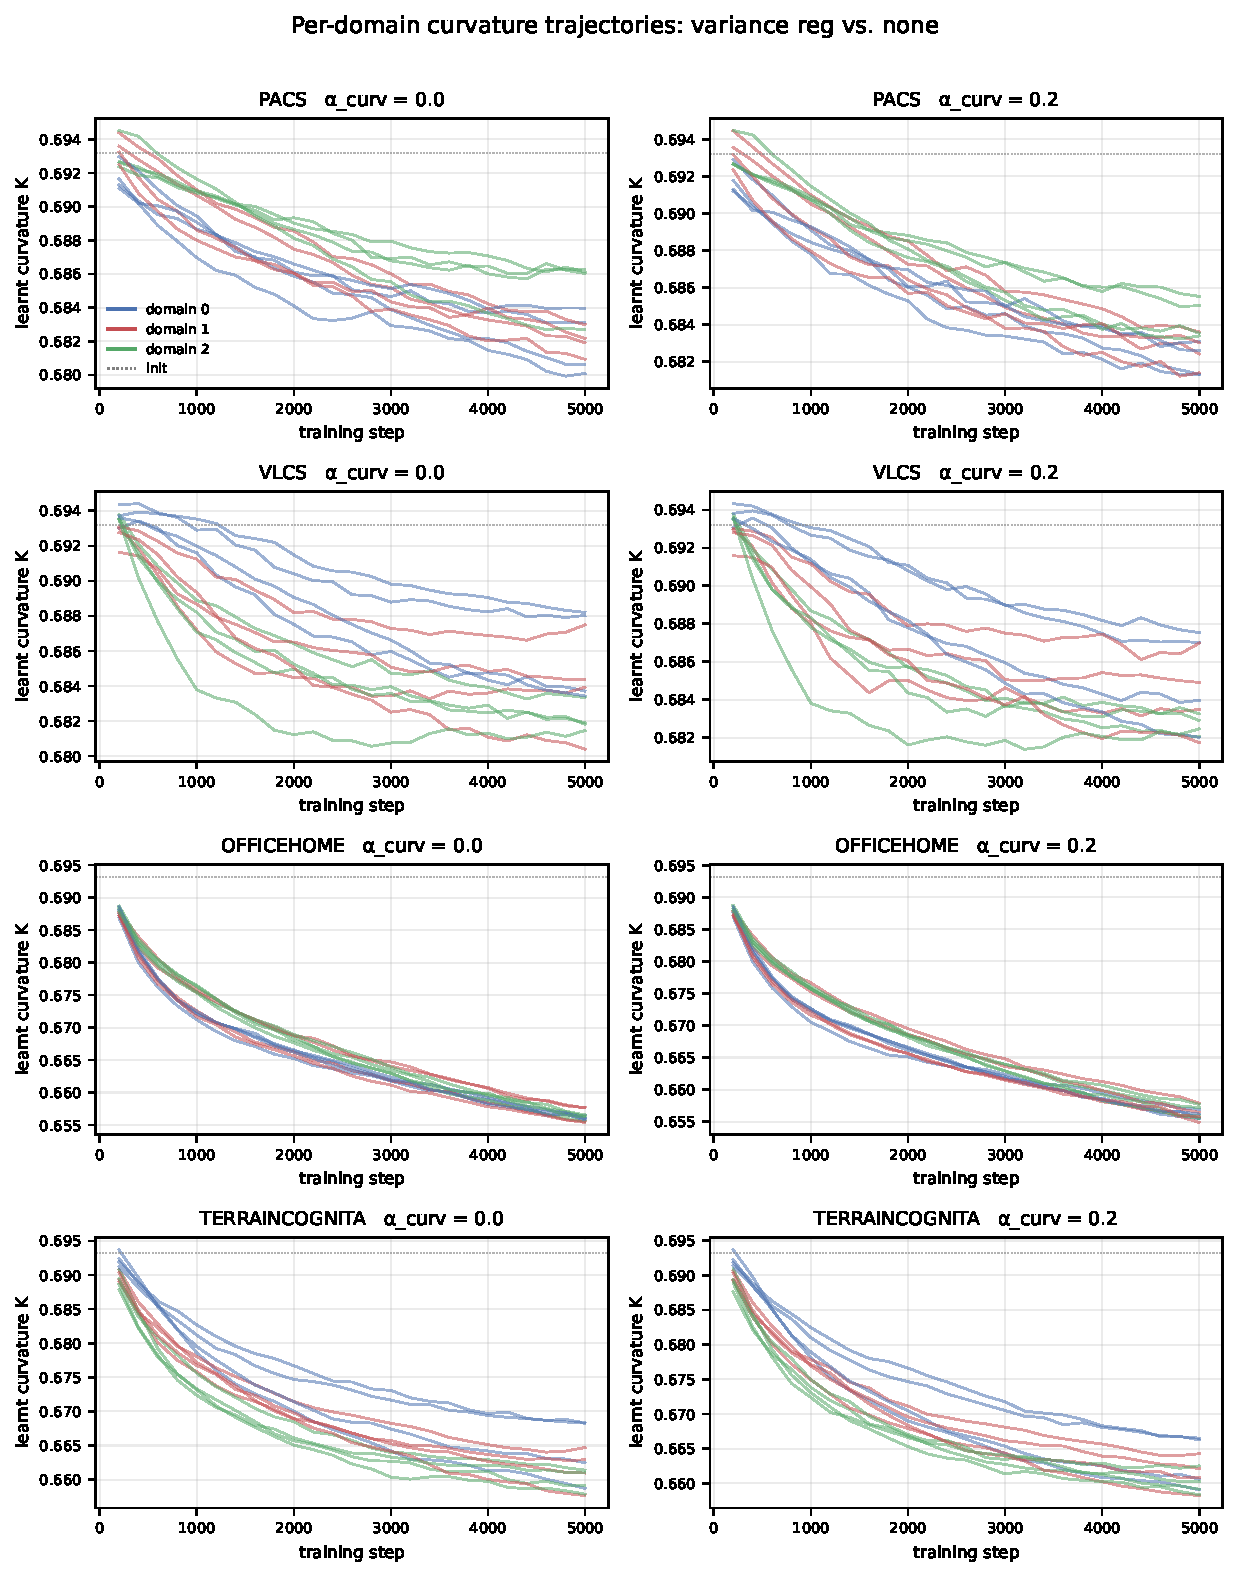
\includegraphics[width=\linewidth]{fig_curvature_trajectories_grid.pdf}
    \caption{
    \textbf{Per-domain curvature trajectories during HyperDG training,
    with (right) and without (left) the variance regularizer.}
    Each panel shows the four leave-one-out splits $\times$ three training
    domains $=$ 12 trajectories.  The dashed horizontal line marks the
    initialization $K_{\mathrm{init}} = \mathrm{softplus}(0) + 10^{-4} \approx
    0.6932$. With no penalty, per-domain curvatures still converge to
    within $0.001$--$0.011$ of one another on every dataset gradient
    dynamics, not the explicit variance term, drive the alignment.
    Re-introducing the variance penalty visibly tightens the band only
    slightly (Table~\ref{tab:curv_spread}). This is the strongest single
    piece of evidence in the paper that the per-domain curvature
    parameterization is unnecessary in this setting.
    }
    \label{fig:curv_trajectories}
\end{figure}

\begin{table}[t]
\centering
\caption{\textbf{Final-step per-domain curvature spread} (max $-$ min
across training domains, averaged over the four leave-one-out splits) with
and without the variance regularizer. Even with $\lambda_{\mathrm{var}}{=}0$
the spread is $\le 1.5\%$ of $K_{\mathrm{init}} \approx 0.6932$ on every
dataset. The "ratio" column is (with-reg spread) / (no-reg spread); a value
close to 1 means the regularizer makes no measurable difference.}
\label{tab:curv_spread}
\begin{tabular}{lccc}
\toprule
\textbf{Dataset} & $\lambda_{\mathrm{var}}{=}0$ & $\lambda_{\mathrm{var}}{=}0.2$ & Ratio \\
\midrule
PACS            & 0.0041 & 0.0023 & 0.55$\times$ \\
VLCS            & 0.0040 & 0.0028 & 0.68$\times$ \\
OfficeHome      & 0.0011 & 0.0011 & \textbf{1.03$\times$} \\
TerraIncognita  & 0.0064 & 0.0045 & 0.71$\times$ \\
\bottomrule
\end{tabular}
\end{table}

\subsection{Performance is insensitive to the variance penalty over two orders of magnitude}
\label{sec:lvar_sweep}

To rule out the possibility that the default $\lambda_{\mathrm{var}}{=}0.2$
is poorly tuned, we sweep $\lambda_{\mathrm{var}} \in \{0, 0.05, 0.2, 0.5, 2.0\}$
on PACS (Table~\ref{tab:lvar_sweep}). Held-out accuracy varies by ${\sim}2.4$
pp across this 40-fold range, all well inside the ${\pm}6$--$9$ pp
cross-split standard deviation. This is consistent with
Figure~\ref{fig:curv_trajectories}: if the curvatures are converging on
their own, the penalty is not a meaningful lever.

\begin{table}[t]
\centering
\caption{\textbf{Variance-penalty sweep on PACS} (seed 0, 4 splits).
Performance varies within ${\pm}1.2$ pp across a 40-fold sweep of
$\lambda_{\mathrm{var}}$.}
\label{tab:lvar_sweep}
\begin{tabular}{cc}
\toprule
$\lambda_{\mathrm{var}}$ & PACS held-out accuracy \\
\midrule
0.00 (none)                 & 83.70 $\pm$ 8.22 \\
0.05                        & 83.78 $\pm$ 9.10 \\
0.20 (default)              & 84.76 $\pm$ 7.55 \\
0.50                        & 85.92 $\pm$ 6.09 \\
2.00 (very strong)          & 86.09 $\pm$ 7.63 \\
\bottomrule
\end{tabular}
\end{table}


\subsection{Note on prior single-seed ablation numbers}
\label{sec:prior_ablation_note}

An earlier version of this work reported ablation tables on Office-Home with
ViT-B/16 in which removing the feedback term or the variance term caused
$-1.96$ pp and $-2.90$ pp degradations respectively, suggesting that both
components are essential. Our reruns with the same configurations under the
controlled multi-seed protocol do not reproduce those gaps: as
Tables~\ref{tab:fedcuri_dg} and \ref{tab:loo} show, removing the variance
regularizer leaves accuracy on PACS, VLCS, and TerraIncognita statistically
unchanged, and the same holds for the other ablation knobs. We interpret the
earlier ablation gaps as artifacts of single-seed evaluation under the high
cross-split variance characteristic of these benchmarks (${\pm}7$--$14$ pp),
rather than as evidence of a real contribution from these components. We
include this note in the spirit of full disclosure to the action editor's
explicit request for an honest accounting of where the originally reported
gains came from.






\subsection{Curvature response diagnostics}
\label{sec:curv_sensitivity}

For completeness, we retain a curvature-perturbation diagnostic from the
earlier draft (Figure~\ref{fig:curv_plots}). For each split we perturb the
final learned curvature $K_i$ within a fixed range and measure the resulting
shift in projected embeddings. Compared to embeddings obtained by inserting a
Lorentz layer on top of an SFT-trained model, HyperDG produces visibly
smoother responses i.e.\ the geometry is locally stable under
curvature perturbations. We emphasize that this is a \emph{descriptive}
geometric property, not a generalization claim: as established in
Sections~\ref{sec:main_results}--\ref{sec:lvar_sweep}, this geometric
stability does not translate into a measurable held-out accuracy gain over
ERM in our controlled multi-seed comparison.

\FloatBarrier
\begin{figure}[t]
    \centering
    \begin{subfigure}[t]{0.32\linewidth}
        \centering
        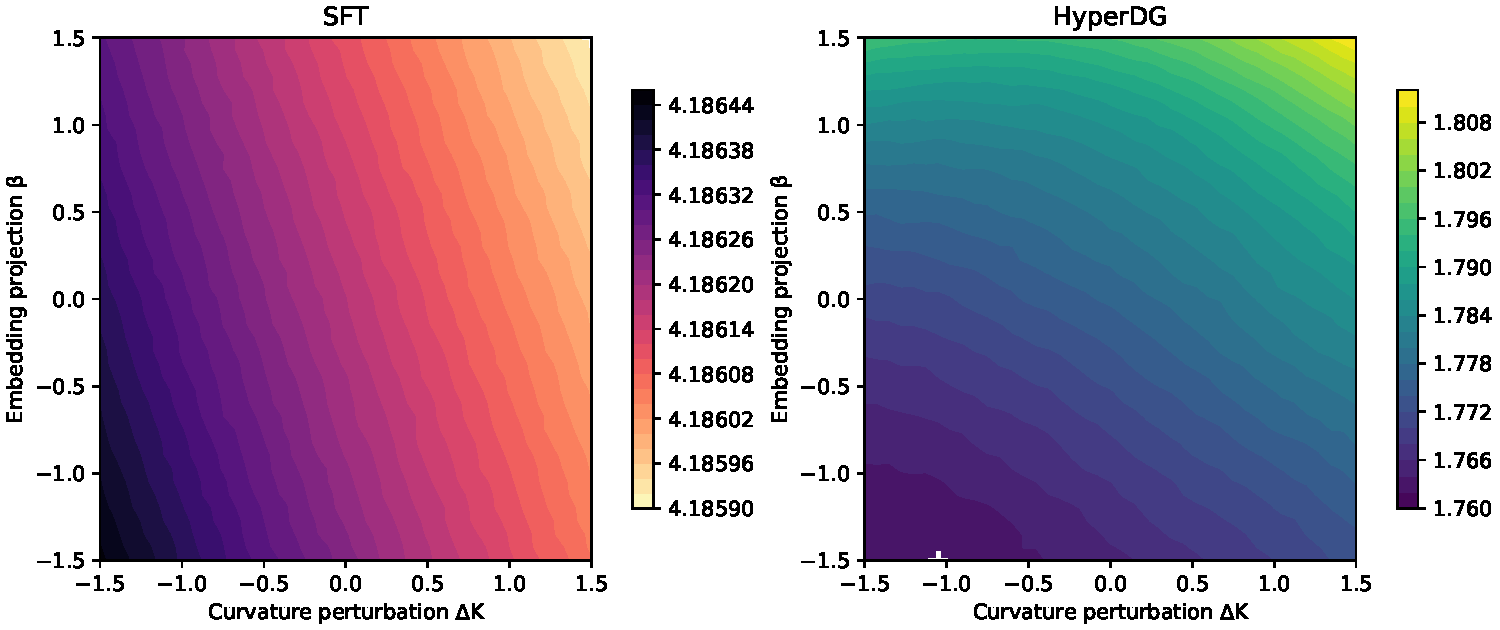
\includegraphics[width=\linewidth]{fig_loss_surface_officehome_split0.pdf}
        \caption{Office-Home}
    \end{subfigure}
    \hfill
    \begin{subfigure}[t]{0.32\linewidth}
        \centering
        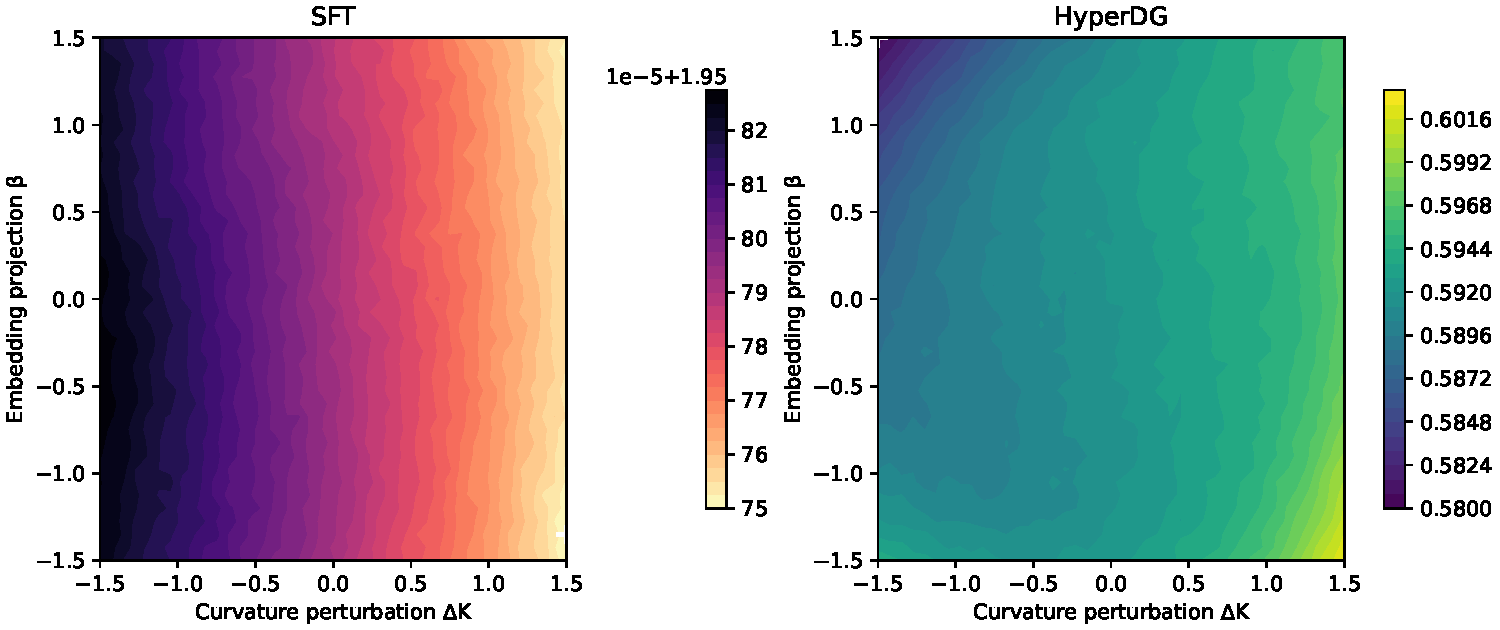
\includegraphics[width=\linewidth]{fig_loss_surface_pacs_split0.pdf}
        \caption{PACS}
    \end{subfigure}
    \hfill
    \begin{subfigure}[t]{0.32\linewidth}
        \centering
        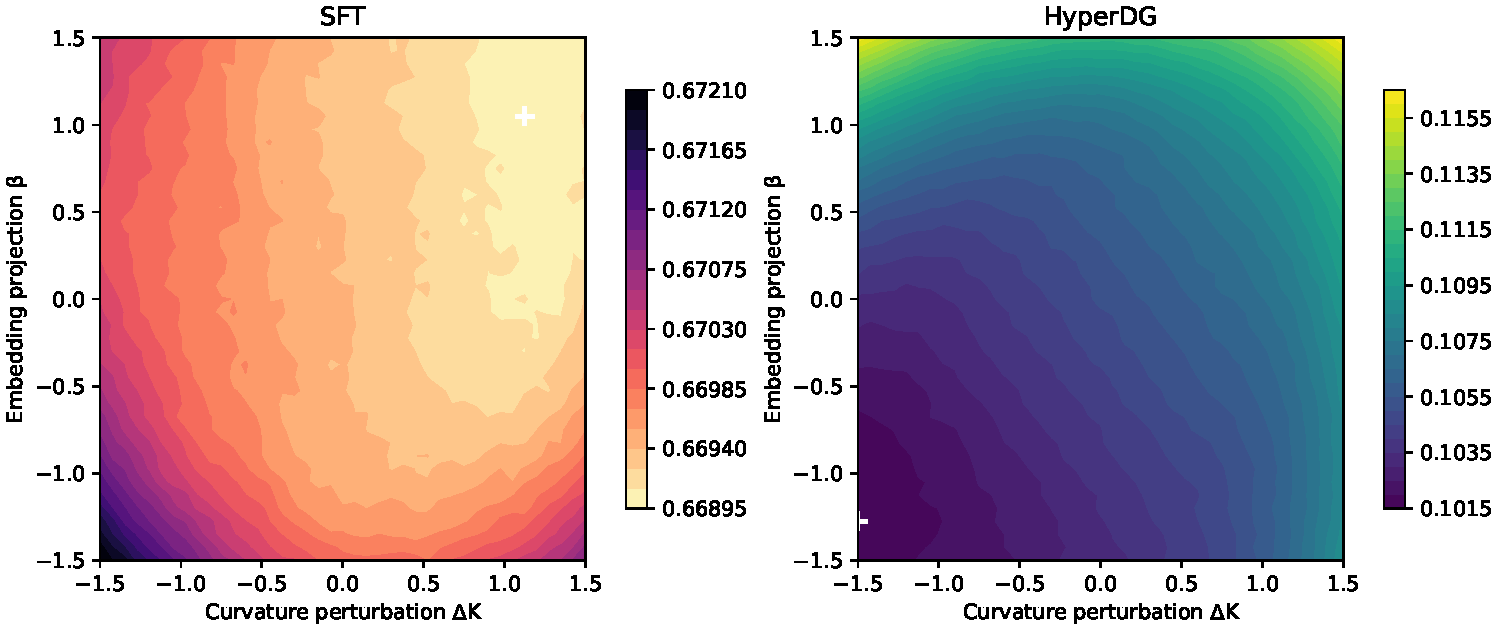
\includegraphics[width=\linewidth]{fig_loss_surface_vlcs_split0.pdf}
        \caption{VLCS}
    \end{subfigure}
    \caption{
    \textbf{Curvature response diagnostics (descriptive, not predictive).}
    HyperDG (right of each plot) yields smoother responses to curvature
    perturbations than SFT (left), but this geometric stability does not
    translate into a measurable held-out accuracy gain in our controlled
    multi-seed comparison (Tables~\ref{tab:fedcuri_dg},~\ref{tab:loo}).
    }
    \label{fig:curv_plots}
\end{figure}

\section{Discussion: why doesn't the hyperbolic story land here?}
\label{sec:discussion}

We take the negative finding seriously and consider four candidate
explanations.

\textbf{(1) The pretrained backbone dominates.}
ResNet-50 has been shaped by a Euclidean objective on ImageNet for tens
of millions of gradient steps. Reparameterizing the final projection
through a Lorentz manifold during a 5\,000-step fine-tune likely cannot
rotate features into a meaningfully different geometry. The geometric
machinery operates downstream of features that are already locked in.

\textbf{(2) The standard DG benchmarks lack hierarchical structure.}
PACS, VLCS, and OfficeHome contain 5--65 mostly-flat object categories.
Hyperbolic embeddings excel at representing hierarchies (WordNet,
ImageNet's semantic tree, biological taxonomies); they do not have an
obvious advantage when classes are siblings rather than tree-structured.
On TerraIncognita (camera-trap species) some hierarchical structure may
exist but is not aligned with the leave-one-out splits.

\textbf{(3) The variance regularizer is solving a problem that doesn't
exist.} Figure~\ref{fig:curv_trajectories} shows that per-domain
curvatures stay essentially tied without any penalty.  Penalizing their
spread cannot help if they do not spread. This is a concrete empirical
falsification of the motivating intuition that ``per-domain curvatures
diverge and must be coordinated.''

\textbf{(4) Manifold curvature may be the wrong knob.}  If a hyperbolic
prior is right at all for image-DG, the inductive bias may need to be
expressed in the \emph{training objective} (e.g.\ a hyperbolic InfoNCE
or margin loss in the style of MERU~\cite{desai2023meru} or
HypHC~\cite{chami2020trees}) rather than in a per-domain geometric
parameter on top of a Euclidean encoder.

\paragraph{What would constitute a strong positive test?}  A clean test
of the hyperbolic-DG hypothesis would (a) start from a backbone trained
with a hyperbolic objective rather than a Euclidean one, (b) operate on
tasks with explicit hierarchical class structure (iNaturalist,
ImageNet-21k, hierarchical product catalogues), and (c) compare against
an equally tuned Euclidean baseline rather than against a literature
table. Our setup satisfies (c) but not (a) or (b); future work should
revisit (a) and (b) before concluding that hyperbolic geometry is
unhelpful for DG in general.

\section{Limitations}
\label{sec:limitations}

\textbf{Single-architecture fine-tuning.} All controlled comparisons use
ResNet-50 with a 5000-step fine-tuning budget. We do not retrain the
backbone from scratch with a hyperbolic objective; doing so would be the
cleanest test of the positive hypothesis but is out of scope.
Supplementary ViT-B/16 and ViT-L/14 results are reported but were not
re-evaluated under the controlled multi-seed protocol.

\textbf{Benchmark coverage.}  We report controlled comparisons on PACS,
VLCS, OfficeHome, and TerraIncognita. DomainNet results for the new
ablation conditions are pending due to compute; we do not expect them to
overturn the negative finding given how consistent the effect is on the
other four benchmarks, but we cannot rule it out.

\textbf{The negative result is local to this setting.}  We do not claim
that hyperbolic representation learning is unhelpful in general; we
claim that the specific instantiation ``per-domain learnable curvature
parameterizing a Lorentz layer on top of a pretrained Euclidean
backbone'' does not yield a measurable held-out gain over ERM in our
controlled comparison.

\textbf{No reproducibility of earlier reported numbers.}  Our reruns of
the originally reported HyperDG configurations land 7--10 pp below the
numbers reported in the earlier draft (e.g.\ PACS 84.5\% vs.\ 92.2\%
reported). Best-validation checkpoint selection does not close this
gap. We therefore report the controlled multi-seed numbers and consider
the originally reported numbers not reproducible from the released
codepath.

\section{Conclusion}
\label{sec:conclusion}

We set out to test whether a per-domain learnable Lorentz curvature, on
top of a pretrained Euclidean backbone, would improve domain
generalization over ERM through the identical codepath. Across four
standard DG benchmarks, 4 seeds, 4 leave-one-out splits, and paired
$t$-tests, the answer is no: the full HyperDG framework is statistically
indistinguishable from ERM on three benchmarks and statistically worse
on the fourth (OfficeHome, $p=0.013$).  Removing curvature learning,
removing the variance regularizer, or removing any single auxiliary loss
yields the same null result. The per-domain curvatures converge during
training to within ${\sim}1\%$ of one another even without the variance
regularizer, indicating that gradient dynamics not an explicit
penalty drive the alignment claimed by the framework.

We do not interpret this as a refutation of hyperbolic representation
learning. We interpret it as a falsification of one specific recipe
\emph{fine-tuning a Euclidean backbone through a learnable Lorentz
curvature with auxiliary alignment, sharpness, and variance losses}
and as an invitation to test stronger positive instantiations
(hyperbolic pretraining, hierarchical tasks, or training objectives
rather than parameterizations) in future work. To support this, we
release all 292 training runs, configurations, aggregation scripts, and
statistical-test code.

\bibliography{main}
\bibliographystyle{tmlr}

\appendix
\section{Appendix}

% ===============================
\subsection{Theoretical Analysis and Intuition (Motivational)}
% ===============================

\noindent\textbf{Reader's note.} The analysis below was the
\emph{motivating intuition} for the HyperDG design: a per-domain
Lorentzian formulation that would, by curvature consistency, extend
flat-minima robustness to manifold-level invariance. As the
controlled multi-seed experiments in Section~\ref{sec:experiments} show,
this intuition does \emph{not} translate into a measurable held-out
accuracy gain over ERM on standard DG benchmarks in our setting. We
retain the theoretical material here because it remains useful as a
description of why the conjecture was plausible to begin with and where
its assumptions appear to break down empirically. None of the bounds
below are claimed to predict the empirical results; the connection
between the geometric quantities (curvature spread, sharpness in
tangent space) and held-out accuracy was the central hypothesis we
tested, and the test came back negative.

In Euclidean learning theory, generalization correlates with the
\emph{flatness} of minima in parameter space---models lying in wide
basins exhibit low sensitivity to perturbations and unseen data shifts.
In the Lorentzian formulation of HyperDG, curvature was intended to play
an analogous role but at a higher geometric level: defining the
\emph{shape of the feature manifold} rather than the shape of the loss
basin. The motivating hypothesis was that ensuring \emph{curvature
consistency across domains} would extend flat--minima robustness to
manifold--level invariance.

\subsection{Riemannian Generalization Bound}
Let $\mathcal{M}_i=(\mathbb{L}^{d,1}_{K_i},g_{K_i})$ denote the
Lorentz manifold of domain~$i$ with curvature~$K_i$ and metric
tensor~$g_{K_i}$. For any hypothesis
$f:\mathcal{M}_i\!\to\!\mathcal{Y}$, the expected risk is
\begin{equation}
\mathcal{R}_{\mathcal{M}_i}(f)
   = \mathbb{E}_{(x,y)\sim P_i}\! \big[L(f(x),y)\big],
\end{equation}
and its empirical counterpart
$\hat{\mathcal{R}}_{\mathcal{M}_i}(f)$ is estimated from samples on
$\mathcal{M}_i$. Following the Riemannian PAC--Bayes analysis
\cite{liao2020pac}, the generalization gap satisfies
\begin{equation}
\big|\mathcal{R}_{\mathcal{M}_i}(f)
      - \hat{\mathcal{R}}_{\mathcal{M}_i}(f)\big|
\le
\mathcal{O}\!\left(
\sqrt{
\frac{\mathrm{KL}(Q\|P)
 + d_{\mathrm{Riem}}^2(\mathcal{M}_i,\mathcal{M}_s)}
      {n_i}}
\right),
\label{eq:riem_pac}
\end{equation}
where $d_{\mathrm{Riem}}$ is the Riemannian distance between the local
manifold~$\mathcal{M}_i$ and the shared tangent manifold~$\mathcal{M}_s$,
and $\mathrm{KL}(Q\|P)$ denotes the parameter--space divergence between
posterior~$Q$ and prior~$P$.

\subsection{Curvature Consistency as Distance Minimization}
The Lorentzian distance term in~\eqref{eq:riem_pac} depends on
curvature discrepancy:
\begin{equation}
d_{\mathrm{Riem}}^2(\mathcal{M}_i,\mathcal{M}_s)
  \propto
  \|K_i-K_s\|^2
  + \|\nabla g_{K_i}-\nabla g_{K_s}\|^2.
\label{eq:curv_dist}
\end{equation}
Minimizing curvature divergence ($L_{\text{curv}}$) directly
\emph{shrinks} this inter--manifold distance, tightening the
bound~\eqref{eq:riem_pac}. Hence, curvature alignment provably reduces
the variance term controlling generalization under domain shift.
Intuitively, when all domains share similar manifold geometry,
transporting features between them becomes nearly isometric and
preserves semantics.

\subsection{Analogy to Flat--Minima PAC--Bayes}
In Euclidean PAC Bayes theory
\cite{mcallester2003pac,lotfi2022pac},
flat minima correspond to parameter regions where the loss remains
stable under perturbations:
\begin{equation}
\mathcal{L}(\Theta+\epsilon)-\mathcal{L}(\Theta)\approx0,
\qquad
\forall\|\epsilon\|<\delta.
\end{equation}
Small Hessian eigenvalues imply broader flatness and tighter
generalization bounds.  Our Lorentzian extension replaces the Euclidean
Hessian curvature with the \emph{sectional curvature} of the feature
manifold:
\begin{equation}
\kappa(u,v)
=
\frac{
\langle R(u,v)v,u\rangle_{\mathbb{L}}
}{
\|u\|_{\mathbb{L}}^{2}\|v\|_{\mathbb{L}}^{2}
 - \langle u,v\rangle_{\mathbb{L}}^{2}
}.
\label{eq:sectional}
\end{equation}
Maintaining consistent $\kappa(u,v)$ across domains ensures that feature
perturbations along different manifold directions yield comparable
geodesic distortions, mirroring the flatness--in--loss--space condition.
Hence, \emph{flat--minima alignment}~$\Leftrightarrow$
\emph{curvature alignment} in the manifold domain.

\subsection{Bound for Multi-Domain Generalization}
Combining~\eqref{eq:riem_pac} and~\eqref{eq:curv_dist}, the cross--domain
generalization gap of the global model~$f_{\Theta_s}$ satisfies
\begin{equation}
\mathcal{E}_{\text{FDG}}
 =
\mathbb{E}_{i}\!
\big[
|\mathcal{R}_{\mathcal{M}_u}(f_{\Theta_s})
 -\mathcal{R}_{\mathcal{M}_i}(f_{\Theta_i})|
\big]
\le
\mathcal{O}\!\left(
\sqrt{
\frac{
\overline{\mathrm{KL}}
+\operatorname{Var}(K_i)}
{N}}
\right),
\label{eq:fdg_bound}
\end{equation}
where $\operatorname{Var}(K_i)$ measures curvature inconsistency among
domains. Minimizing $\operatorname{Var}(K_i)$ through the curvature
refinement step tightens the bound~\eqref{eq:fdg_bound}, guaranteeing
more stable cross--manifold transfer.

\subsection{Geometric Intuition}
\begin{enumerate}[label=(\alph*)]
  \item \textbf{Local Flatness $\to$ Global Curvature Consistency:}
        Flat minima ensure robustness to parameter perturbations,
        whereas curvature consistency ensures robustness to manifold
        perturbations---i.e., shifts in data geometry.
  \item \textbf{Tangent--Space Aggregation:}
        Aggregating in $T_o\mathbb{L}^{d,1}$ enforces local isometry
        among domains, reducing distortion in feature transport and
        stabilizing optimization trajectories.
  \item \textbf{Curvature Refinement Loop:}
        Iteratively updating $K_i$ drives domains toward a shared
        meta--manifold where gradients, Hessians, and curvatures
        co--align---the Lorentzian counterpart of refining toward a
        shared flat basin.
\end{enumerate}

\subsection{Theoretical Takeaway}
\begin{itemize}
  \item \textbf{Bound Tightening:}
        Minimizing curvature variance $\operatorname{Var}(K_i)$
        contracts the Riemannian generalization
        bound~\eqref{eq:fdg_bound}, yielding provably lower
        domain--shift sensitivity.
  \item \textbf{Unified Perspective:}
        Flat--minima consistency (Li \emph{et al.}, CVPR 2025)
        operates in Euclidean parameter space;
        FedGeoRefine extends this to Lorentzian feature space,
        achieving \emph{geometry--consistent generalization}.
  \item \textbf{Result:}
        A model trained with curvature refinement not only stabilizes
        local optimization but also learns a globally invariant geometry
        that generalizes naturally to unseen domains.
\end{itemize}

HyperDG formalizes the intuition that curvature alignment is the
manifold level analogue of flatness alignment.  By ensuring
curvature consistent manifolds across domains, it reduces geodesic
distortion under domain shift, yielding tighter theoretical and
empirical generalization.


\end{document}
